% Options for packages loaded elsewhere
% Options for packages loaded elsewhere
\PassOptionsToPackage{unicode}{hyperref}
\PassOptionsToPackage{hyphens}{url}
\PassOptionsToPackage{dvipsnames,svgnames,x11names}{xcolor}
%
\documentclass[
  letterpaper,
  DIV=11,
  numbers=noendperiod]{scrreport}
\usepackage{xcolor}
\usepackage{amsmath,amssymb}
\setcounter{secnumdepth}{2}
\usepackage{iftex}
\ifPDFTeX
  \usepackage[T1]{fontenc}
  \usepackage[utf8]{inputenc}
  \usepackage{textcomp} % provide euro and other symbols
\else % if luatex or xetex
  \usepackage{unicode-math} % this also loads fontspec
  \defaultfontfeatures{Scale=MatchLowercase}
  \defaultfontfeatures[\rmfamily]{Ligatures=TeX,Scale=1}
\fi
\usepackage{lmodern}
\ifPDFTeX\else
  % xetex/luatex font selection
\fi
% Use upquote if available, for straight quotes in verbatim environments
\IfFileExists{upquote.sty}{\usepackage{upquote}}{}
\IfFileExists{microtype.sty}{% use microtype if available
  \usepackage[]{microtype}
  \UseMicrotypeSet[protrusion]{basicmath} % disable protrusion for tt fonts
}{}
\makeatletter
\@ifundefined{KOMAClassName}{% if non-KOMA class
  \IfFileExists{parskip.sty}{%
    \usepackage{parskip}
  }{% else
    \setlength{\parindent}{0pt}
    \setlength{\parskip}{6pt plus 2pt minus 1pt}}
}{% if KOMA class
  \KOMAoptions{parskip=half}}
\makeatother
% Make \paragraph and \subparagraph free-standing
\makeatletter
\ifx\paragraph\undefined\else
  \let\oldparagraph\paragraph
  \renewcommand{\paragraph}{
    \@ifstar
      \xxxParagraphStar
      \xxxParagraphNoStar
  }
  \newcommand{\xxxParagraphStar}[1]{\oldparagraph*{#1}\mbox{}}
  \newcommand{\xxxParagraphNoStar}[1]{\oldparagraph{#1}\mbox{}}
\fi
\ifx\subparagraph\undefined\else
  \let\oldsubparagraph\subparagraph
  \renewcommand{\subparagraph}{
    \@ifstar
      \xxxSubParagraphStar
      \xxxSubParagraphNoStar
  }
  \newcommand{\xxxSubParagraphStar}[1]{\oldsubparagraph*{#1}\mbox{}}
  \newcommand{\xxxSubParagraphNoStar}[1]{\oldsubparagraph{#1}\mbox{}}
\fi
\makeatother


\usepackage{longtable,booktabs,array}
\usepackage{calc} % for calculating minipage widths
% Correct order of tables after \paragraph or \subparagraph
\usepackage{etoolbox}
\makeatletter
\patchcmd\longtable{\par}{\if@noskipsec\mbox{}\fi\par}{}{}
\makeatother
% Allow footnotes in longtable head/foot
\IfFileExists{footnotehyper.sty}{\usepackage{footnotehyper}}{\usepackage{footnote}}
\makesavenoteenv{longtable}
\usepackage{graphicx}
\makeatletter
\newsavebox\pandoc@box
\newcommand*\pandocbounded[1]{% scales image to fit in text height/width
  \sbox\pandoc@box{#1}%
  \Gscale@div\@tempa{\textheight}{\dimexpr\ht\pandoc@box+\dp\pandoc@box\relax}%
  \Gscale@div\@tempb{\linewidth}{\wd\pandoc@box}%
  \ifdim\@tempb\p@<\@tempa\p@\let\@tempa\@tempb\fi% select the smaller of both
  \ifdim\@tempa\p@<\p@\scalebox{\@tempa}{\usebox\pandoc@box}%
  \else\usebox{\pandoc@box}%
  \fi%
}
% Set default figure placement to htbp
\def\fps@figure{htbp}
\makeatother

\ifLuaTeX
  \usepackage{luacolor}
  \usepackage[soul]{lua-ul}
\else
  \usepackage{soul}
\fi

% definitions for citeproc citations
\NewDocumentCommand\citeproctext{}{}
\NewDocumentCommand\citeproc{mm}{%
  \begingroup\def\citeproctext{#2}\cite{#1}\endgroup}
\makeatletter
 % allow citations to break across lines
 \let\@cite@ofmt\@firstofone
 % avoid brackets around text for \cite:
 \def\@biblabel#1{}
 \def\@cite#1#2{{#1\if@tempswa , #2\fi}}
\makeatother
\newlength{\cslhangindent}
\setlength{\cslhangindent}{1.5em}
\newlength{\csllabelwidth}
\setlength{\csllabelwidth}{3em}
\newenvironment{CSLReferences}[2] % #1 hanging-indent, #2 entry-spacing
 {\begin{list}{}{%
  \setlength{\itemindent}{0pt}
  \setlength{\leftmargin}{0pt}
  \setlength{\parsep}{0pt}
  % turn on hanging indent if param 1 is 1
  \ifodd #1
   \setlength{\leftmargin}{\cslhangindent}
   \setlength{\itemindent}{-1\cslhangindent}
  \fi
  % set entry spacing
  \setlength{\itemsep}{#2\baselineskip}}}
 {\end{list}}
\usepackage{calc}
\newcommand{\CSLBlock}[1]{\hfill\break\parbox[t]{\linewidth}{\strut\ignorespaces#1\strut}}
\newcommand{\CSLLeftMargin}[1]{\parbox[t]{\csllabelwidth}{\strut#1\strut}}
\newcommand{\CSLRightInline}[1]{\parbox[t]{\linewidth - \csllabelwidth}{\strut#1\strut}}
\newcommand{\CSLIndent}[1]{\hspace{\cslhangindent}#1}



\setlength{\emergencystretch}{3em} % prevent overfull lines

\providecommand{\tightlist}{%
  \setlength{\itemsep}{0pt}\setlength{\parskip}{0pt}}



 


% gt_packages.sty
\usepackage{multirow}    % For multirow cells
\usepackage{colortbl}    % For colored cells in tables
\usepackage{xcolor}      % For custom colors
\usepackage{array}       % For advanced table formatting
\usepackage{booktabs}    % For professional-looking tables
\usepackage{longtable}   % For tables that span multiple pages
\usepackage{graphicx}    % For including images in tables
\usepackage[backend=biber]{biblatex} % For bibliography management
\usepackage{hyperref}    % For hyperlinks in the document
\usepackage{caption}     % For custom table / figure captions

% Format figure captions  -------------------------------------------------------

\captionsetup[figure]{
  font={small, it},
  labelfont={bf,small,color=gray},
  justification=justified,
  textfont={color=gray},
  aboveskip=10pt,
  belowskip=0pt,
}

\newenvironment{fakecaption}
{
  \begingroup
  \small\itshape\color{gray}
  \setlength{\parskip}{5pt} % Add spacing between paragraphs
  \setlength{\leftskip}{60pt} % Left indented
  \setlength{\rightskip}{0pt} % justified
}
{
  \par
  \endgroup
}

% Format Part titles ------------------------------------------------------------

% \renewcommand\part[1]{} % <-- Remove part page

% Only print part title
\makeatletter
\renewcommand\part[1]{ % <-- Specify that \part takes one argument

    % Remove "Part I"
    % {\centering\normalfont\Huge\bfseries \partname\space\thepart\par}

    \def\temp{#1} % Store title in a temporary variable

    % Add part title to the TOC if it is not empty 
    \ifx\temp\empty
    \else
      % Clear the page 
      \if@openright\cleardoublepage\else\clearpage\fi
      \thispagestyle{plain}
      \vspace*{4\baselineskip} % Adjust vertical spacing

      % Add part title to the TOC
      \addcontentsline{toc}{part}{#1} % <-- Use #1 to insert part title
      
      % Print the part title
      \vspace*{2\baselineskip} % Adjust vertical spacing
      {\centering\normalfont\Huge\bfseries #1\par}
      \vskip 3\baselineskip
    \fi
}
\makeatother

% Format quotes ------------------------------------------------------------

% Custom environment for .quotify divs
\newenvironment{quotify}
{
  \vspace*{\fill} % Add vertical space to center the content
  \begin{flushright} % Align the content to the right
}
{
  \end{flushright}
  \vspace*{\fill} % Add vertical space to center the content
}

% Format headings ------------------------------------------------------------

% Make #### headings italic and reduce space after
\addtokomafont{paragraph}{\itshape} % Make paragraph headings italics

% Format text ------------------------------------------------------------

% \setlength{\parindent}{20pt} % Indentation for paragraphs
\KOMAoption{captions}{tableheading}
\makeatletter
\@ifpackageloaded{tcolorbox}{}{\usepackage[skins,breakable]{tcolorbox}}
\@ifpackageloaded{fontawesome5}{}{\usepackage{fontawesome5}}
\definecolor{quarto-callout-color}{HTML}{909090}
\definecolor{quarto-callout-note-color}{HTML}{0758E5}
\definecolor{quarto-callout-important-color}{HTML}{CC1914}
\definecolor{quarto-callout-warning-color}{HTML}{EB9113}
\definecolor{quarto-callout-tip-color}{HTML}{00A047}
\definecolor{quarto-callout-caution-color}{HTML}{FC5300}
\definecolor{quarto-callout-color-frame}{HTML}{acacac}
\definecolor{quarto-callout-note-color-frame}{HTML}{4582ec}
\definecolor{quarto-callout-important-color-frame}{HTML}{d9534f}
\definecolor{quarto-callout-warning-color-frame}{HTML}{f0ad4e}
\definecolor{quarto-callout-tip-color-frame}{HTML}{02b875}
\definecolor{quarto-callout-caution-color-frame}{HTML}{fd7e14}
\makeatother
\makeatletter
\@ifpackageloaded{bookmark}{}{\usepackage{bookmark}}
\makeatother
\makeatletter
\@ifpackageloaded{caption}{}{\usepackage{caption}}
\AtBeginDocument{%
\ifdefined\contentsname
  \renewcommand*\contentsname{Table of contents}
\else
  \newcommand\contentsname{Table of contents}
\fi
\ifdefined\listfigurename
  \renewcommand*\listfigurename{List of Figures}
\else
  \newcommand\listfigurename{List of Figures}
\fi
\ifdefined\listtablename
  \renewcommand*\listtablename{List of Tables}
\else
  \newcommand\listtablename{List of Tables}
\fi
\ifdefined\figurename
  \renewcommand*\figurename{Figure}
\else
  \newcommand\figurename{Figure}
\fi
\ifdefined\tablename
  \renewcommand*\tablename{Table}
\else
  \newcommand\tablename{Table}
\fi
}
\@ifpackageloaded{float}{}{\usepackage{float}}
\floatstyle{ruled}
\@ifundefined{c@chapter}{\newfloat{codelisting}{h}{lop}}{\newfloat{codelisting}{h}{lop}[chapter]}
\floatname{codelisting}{Listing}
\newcommand*\listoflistings{\listof{codelisting}{List of Listings}}
\makeatother
\makeatletter
\makeatother
\makeatletter
\@ifpackageloaded{caption}{}{\usepackage{caption}}
\@ifpackageloaded{subcaption}{}{\usepackage{subcaption}}
\makeatother
\usepackage{bookmark}
\IfFileExists{xurl.sty}{\usepackage{xurl}}{} % add URL line breaks if available
\urlstyle{same}
\hypersetup{
  pdftitle={under the skin},
  pdfauthor={Serena Defina},
  colorlinks=true,
  linkcolor={blue},
  filecolor={Maroon},
  citecolor={Blue},
  urlcolor={Blue},
  pdfcreator={LaTeX via pandoc}}


\title{under the skin}
\usepackage{etoolbox}
\makeatletter
\providecommand{\subtitle}[1]{% add subtitle to \maketitle
  \apptocmd{\@title}{\par {\large #1 \par}}{}{}
}
\makeatother
\subtitle{Early-life stress exposure and the co-occurrence of mental and
physical health problems}
\author{Serena Defina}
\date{}
\begin{document}
\maketitle


% include Doc committee info in the pdf
\clearpage
\thispagestyle{empty} 
\vspace*{1cm}  % Add vertical space at top of page
\textbf{Doctoral committee}

\vspace{1em}
\textbf{PROMOTOR}\\
\vspace{0.5em}
\hspace*{1cm}Henning Tiemier

\vspace{1em}
\textbf{CO-PROMOTORS}\\
\vspace{0.5em}
\hspace*{1cm}Charlotte A.M. Cecil\\
\vspace{0.5em}
\hspace*{1cm}Janine F. Felix
\clearpage


\bookmarksetup{startatroot}

\chapter*{}\label{section}
\addcontentsline{toc}{chapter}{}

\markboth{}{}

\bookmarksetup{startatroot}

\chapter*{PREFACE}\label{preface}
\addcontentsline{toc}{chapter}{PREFACE}

\markboth{PREFACE}{PREFACE}

\begin{tcolorbox}[enhanced jigsaw, left=2mm, coltitle=black, opacityback=0, colframe=quarto-callout-note-color-frame, breakable, colbacktitle=quarto-callout-note-color!10!white, bottomrule=.15mm, toptitle=1mm, toprule=.15mm, leftrule=.75mm, title=\textcolor{quarto-callout-note-color}{\faInfo}\hspace{0.5em}{Note}, titlerule=0mm, arc=.35mm, bottomtitle=1mm, colback=white, rightrule=.15mm, opacitybacktitle=0.6]

This is a work in progress. Stay tuned :)

\end{tcolorbox}

Dear reader,

Let me begin this book the only way that feels right: with a little note
of honesty. Writing this was hard, much harder than I anticipated.
Perhaps out of pride, or because of this irresistible greed I feel to
dissect and point out limitations - that, I am told, makes for a good
scientist as much as a horrible friend - I kept wondering whether any of
this would be worth your time.

I guess 5-years-ago me hoped, at this point, they could promise you
sensational scientific breakthroughs and game-changing statistical
tricks ahead. Well, it looks like we may both have to settle for a
somewhat less glamourous, but perhaps more truthful, process of
scientific discovery.

So here is a collection of small steps toward understanding, many little
increments of knowledge, a couple of false starts, a few frustratingly
inconclusive results, and a handful of insights (some grim, some
hopeful).

Still here? Didn't think so\ldots{} let's talk about early-life stress,
shall we?

\newpage

\begin{quotify}
\emph{``In the depth of winter, I found there was, within me, an
invincible summer.''} \newline Albert Camus -- Summer (1954)
\end{quotify}

\part{}

\chapter{General Introduction}\label{sec-chapter1}

\section{Early-life stress (ELS)}\label{early-life-stress-els}

When my mother was pregnant with me, my older brother died of a
congenital condition. I never met the little guy, never experienced any
grief myself. Yet, for the longest time I thought that, somehow, his
death had cast a sort of shadow over the rest of my life. And I was not
the only one. The idea that exposure to stressful experiences during
\emph{``critical'' periods} of early development wields profound,
long-term impact on emotional and physiological regulation, is nothing
new. Sigmund Freud, among others, made quite a sensational career out of
it, and - perhaps partly because of the success of psychoanalytic
theories - the scientific literature on the topic today is almost
intimidatingly vast.

So vast in fact, that it requires a pinch of terminology clarification,
before we can dive into it. For the remainder of this book, I will use
the term ``Early-Life Stress'' (ELS) to refer to a host of adverse life
events or conditions, that are experienced during the first years of
life, e.g., in childhood, and, even earlier, during gestation. These
experiences (sometimes also referred to as ``childhood trauma'',
``maltreatment'', ``early adversity'', or ``adverse childhood
experiences'') encompass a wide range of stressors, including neglect
and abuse, bereavement, bullying but also poverty, material deprivation
and/or parental psychopathology (Heim, 2020).

ELS is a widely studied concept, partly because it is surprisingly
common: more than half the population experiences at least one form of
ELS before the age of 18 years (Madigan et al., 2024). But more
importantly, ELS is one of strongest, most consistent predictors of
mental health problems later in life, particularly depression (LeMoult
et al., 2020; Li et al., 2016; Li et al., 2023).

Systematic scientific investigations into ELS and its consequences,
really gained momentum in the late 90s, when large-scale epidemiological
studies, began to also highlight a relationship between ELS and an
increased risk of chronic diseases and premature mortality (e.g.
(Felitti et al., 1998)). This line of evidence also proved very robust
over time, so ELS is now a well-recognised risk factor for
cardio-metabolic health problems, including obesity (Danese \& Tan,
2014; Wiss \& Brewerton, 2020), type 2 diabetes (Zhu et al., 2022),
hypertension and cardio-vascular disease (Jacquet-Smailovic et al.,
2022; Jakubowski et al., 2018).

\section{Mental \& physical health: a comorbidity
paradigm}\label{mental-physical-health-a-comorbidity-paradigm}

Interestingly, parallel to this growing interest in the effects of
stress and psychosocial factors on physical health, the early 2000s also
witnessed a surge of epidemiological studies uncovering the relationship
between depression and cardio-metabolic health problems(Luppino et al.,
2010; Penninx et al., 2001; Van der Kooy et al., 2007). Historically,
these two conditions had been largely investigated as separate entities,
each with distinct risk factors and treatment approaches. Their
connection was not entirely overlooked (see for example early
theoretical work by Engel (1977)), but it remained peripheral to
mainstream medical research until relatively recently.

As more evidence accumulated that depression and cardio-metabolic
conditions tend to co-occur (Anwar et al., 2018; Blasco et al., 2020;
Gutiérrez-Rojas et al., 2020), several potential mechanisms have been
proposed to explain this observed comorbidity (Milaneschi et al., 2019).
One possibility is that these conditions share common risk factors, such
as genetic liability for instance, but also ELS exposure, as discussed
above and supported by a recent large scale meta-analysis (Souama et
al., 2023). It is also possible that experiencing depression may
directly increase the risk of developing cardio-metabolic health
problems later in life. For example, in two meta-analyses based on
longitudinal data, depression was found to be risk factor for obesity
and diabetes (Ditmars et al., 2022; Mannan et al., 2016). Other
longitudinal meta-analyses however, have also shown, in turn, that poor
cardio-metabolic health was a robust predictor of later depression (Zhou
et al., 2024), supporting the hypothesis of a bi-directional
relationship.

\section{ELS and psycho-physical health: towards an integrated
approach}\label{els-and-psycho-physical-health-towards-an-integrated-approach}

So far, we have described a triangle of relationships - i.e., between
\emph{a)} ELS and mental health, \emph{b)} ELS and cardio-metabolic
health, and \emph{c)} mental and cardio-metabolic health
(Figure~\ref{fig-thesis-summary} A), which received considerable
attention in the medical literature. This isn't surprising. Depression
and cardio-metabolic conditions are among the leading causes of death
and disability worldwide, shaping an enormous public health burden which
is largely preventable (Anwar et al., 2018). ELS is a promising shared
risk factor, which can be measured years - and even decades - before
clinical symptoms emerge, making it an ideal candidate for informing
early detection and improving the integrated prevention of
psycho-physical health problems.

\begin{figure}[H]

\centering{

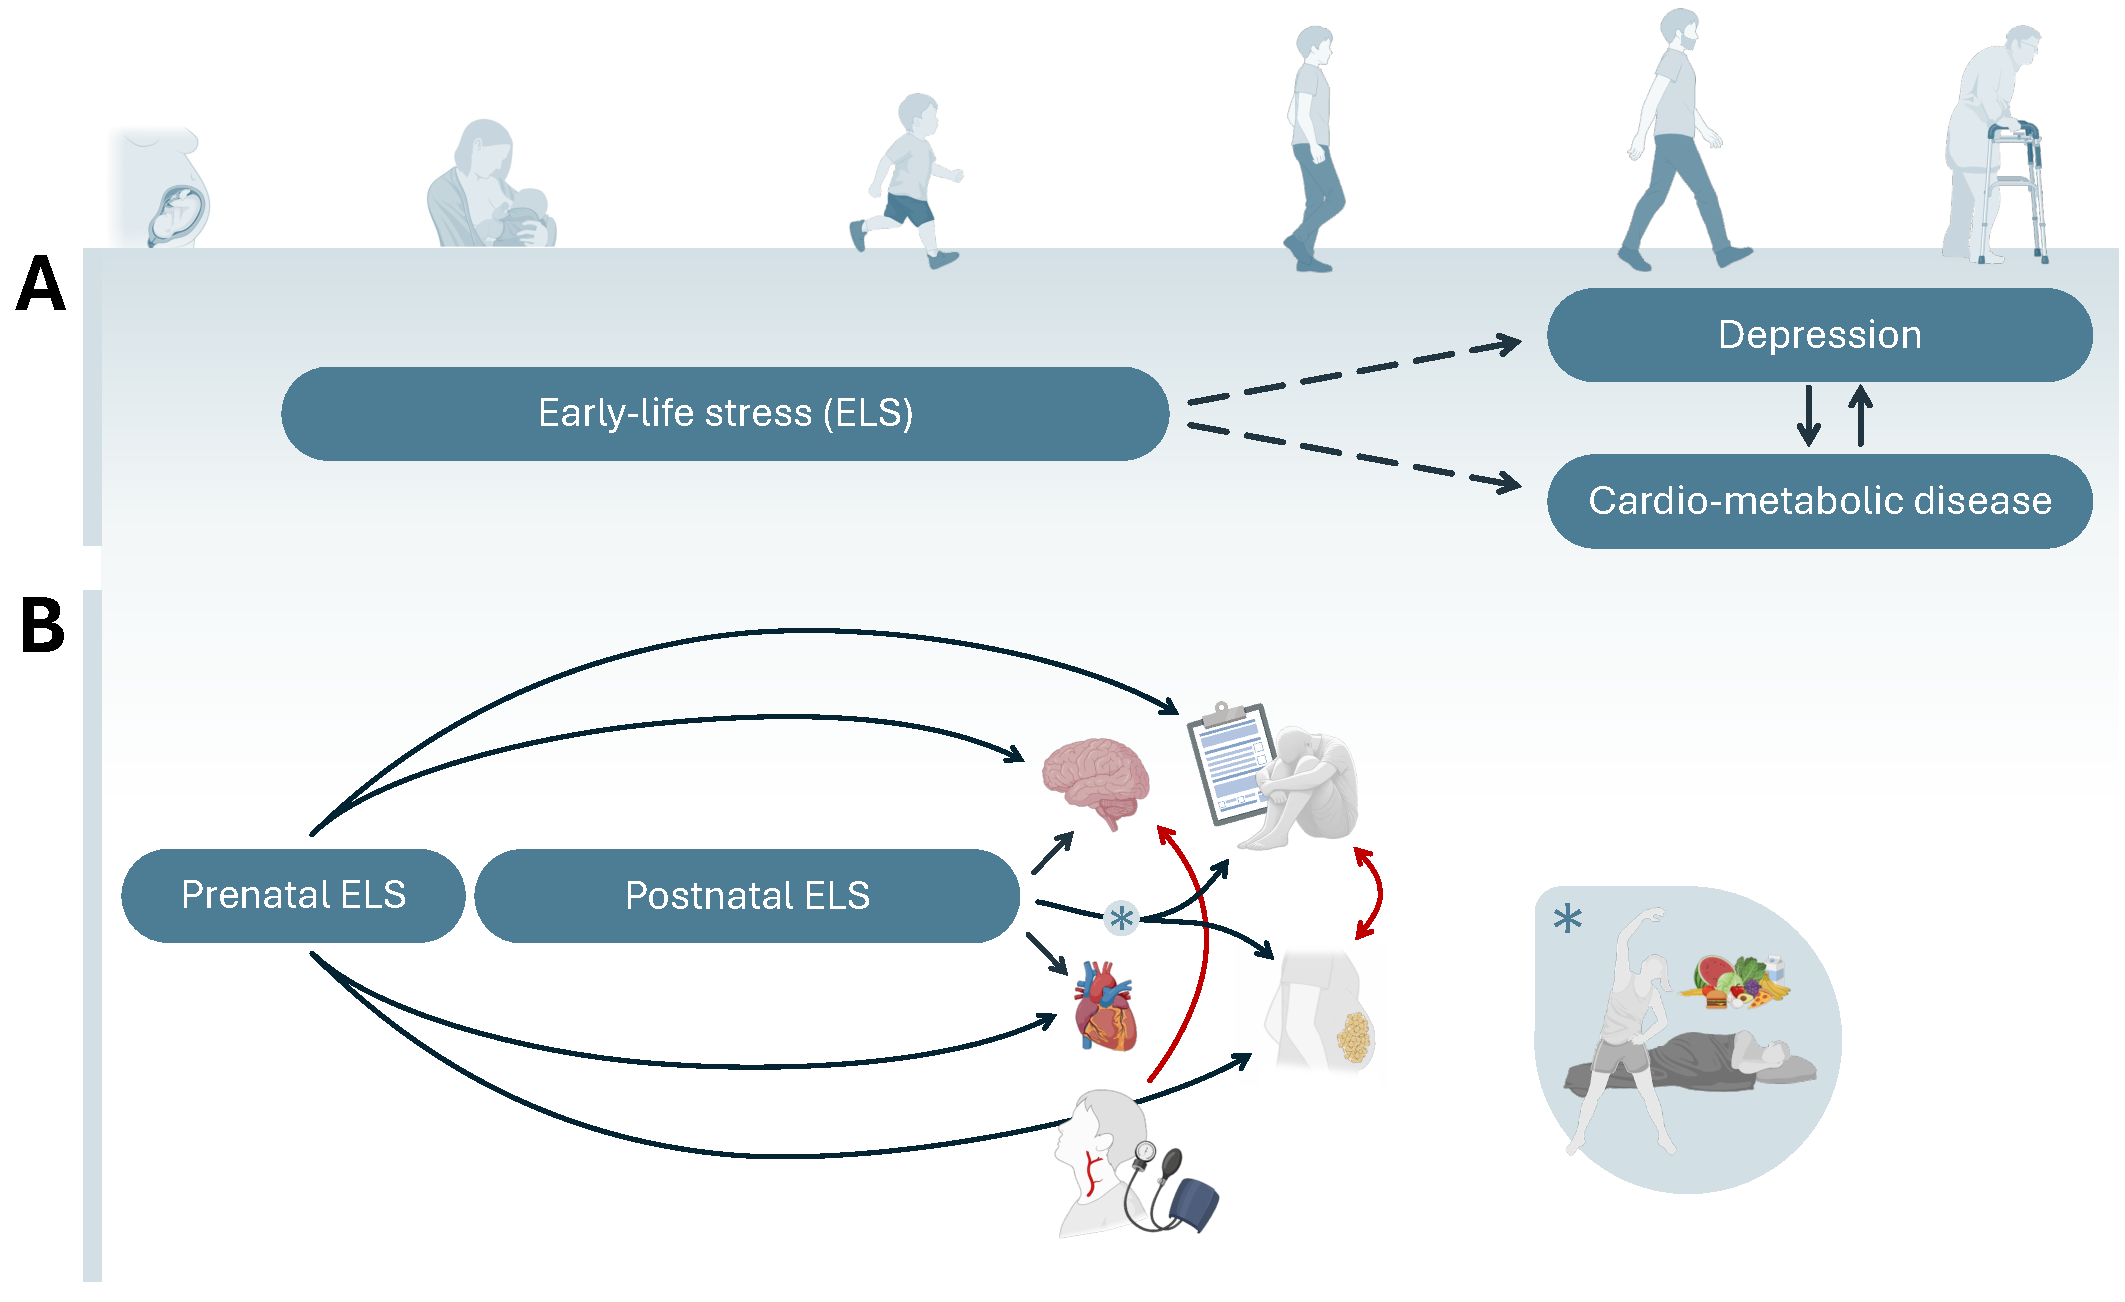
\includegraphics[width=1\linewidth,height=\textheight,keepaspectratio]{1.Introduction/F1_thesissumm.pdf}

}

\caption{\label{fig-thesis-summary}\textbf{Schematic representation of
this thesis, in the context of previous literature}\newline(A) A
schematic summary of the existing evidence, on the relationships under
study. This is largely based on adult outcomes and retrospectively
measured ELS exposure (indicated by the dashed line).\newline(B) A
Schematic summary of the relationships examined in this thesis.}

\end{figure}%

However, there are three key challenges that need to be addressed,
before these findings could be effectively translated into clinical
practice.

Firstly, as briefly noted above, the literature is very heterogenous in
its definition of ELS, with many studies focusing on specific types of
adversity (e.g., childhood neglect and abuse). However, there is
convincing evidence that exposure to multiple stressors - i.e.,
different sources of stress, as well as repeated or continued exposure
over time - has much worse consequences for psycho-physical health,
compared to individual stressors (Evans et al., 2013; Hughes et al.,
2017). This underscores the importance of identifying of children who
face multiple forms of ELS, as they may represent a particularly
vulnerable population, who should be prioritized in intervention
programs.

Secondly, existing studies typically only address one ``side'' of this
triad of relationships. For instance, while ELS has been linked to both
depression and obesity independently, its role in determining their
co-occurrence remains heavily understudied. Consequently, it is hard to
establish the relative importance of ELS as a risk factor for each
disorder in isolation vs.~their comorbidity, which poses an obstacle to
the development of integrated prevention and intervention (Anwar et al.,
2018).

Lastly, the overwhelming majority of studies investigating either the
role of ELS, or the(bidirectional) relationships between mental and
physical health, has been conducted in adult or aging populations.

On one hand, this brings about important measurement issues. Namely, the
proposed relationship between ELS and adult psycho-physical health
relies heavily on retrospective reports of ELS exposure, which may have
introduced recall bias, unrealistically inflating the association
estimates reported by the literature (Reuben et al., 2016).

On the other hand, both depression and cardio-metabolic health problems
very often find their onset well before adulthood. A growing number of
adolescents, for instance, experience depressive symptoms before the age
of 20 years (Keeley, 2021; Patalay \& Gage, 2019). Concurrently, while
cardio-metabolic endpoints such as myocardial infarction and diabetes
are traditionally associated with later life stages, their prodromal
forms, including hypertension, dyslipidemia, and obesity, manifest more
and more frequently between childhood and adolescence (NCD-RisC, 2017;
WHO, 2022). Intervening during this early developmental window could be
crucial to mitigate the progression of such prodromal psycho-physical
symptoms into chronic mental and physical health conditions later in
life.

In this context, prospective cohort studies that begin at conception and
capture a broader spectrum of ELS exposures and psycho-physical
symptoms, are essential to map causal pathways and inform on optimal
intervention windows.

\section{This thesis: one step back in
time}\label{this-thesis-one-step-back-in-time}

This thesis (Figure~\ref{fig-thesis-summary} B) aims to address some of
these limitations and open questions.

\textbf{Part 1} will focus on characterizing the prospective
relationship between ELS and adolescent psycho-physical health. First,
in Chapter~\ref{sec-chapter2}, I quantify the relationship between ELS
exposure during two key developmental periods (i.e.~pregnancy and
childhood) and adolescent \emph{a)} internalizing symptoms, \emph{b)}
adiposity, and \emph{c)} their comorbidity. Chapter~\ref{sec-chapter3}
further explores wether three common lifestyle factors (i.e., physical
activity, sleep duration, and diet quality) may moderate the
associations identified in Chapter~\ref{sec-chapter2}. I will then take
a closer look at the potential ``biological scars'' that pre- and
postnatal ELS exposure may leave behind on children's brains
(Chapter~\ref{sec-chapter4}) and on their hearts
(Chapter~\ref{sec-chapter5}).

In \textbf{Part 2} I will then characterize the reciprocal relationship
between mental and cardio-metabolic health across childhood and
adolescence. Chapter~\ref{sec-chapter6} examines the longitudinal
co-development of depressive symptoms and several markers of
cardio-metabolic health from childhood to early adulthood. In
Chapter~\ref{sec-chapter7}, I assess the relationship between early
cardio-vascular health markers (i.e., arterial health and blood
pressure) and the developing brain.

\section*{References}\label{references}
\addcontentsline{toc}{section}{References}

\markright{References}

\phantomsection\label{refs--1}
\begin{CSLReferences}{1}{0}
\bibitem[\citeproctext]{ref-Anwar2018}
Anwar, N., Kuppili, P. P., \& Balhara, Y. P. S. (2018). Depression and
physical noncommunicable diseases: The need for an integrated approach
{[}Journal Article{]}. \emph{WHO South-East Asia Journal of Public
Health}, \emph{6}(1), 12--17.

\bibitem[\citeproctext]{ref-Blasco2020}
Blasco, B. V., García-Jiménez, J., Bodoano, I., \& Gutiérrez-Rojas, L.
(2020). Obesity and depression: Its prevalence and influence as a
prognostic factor: A systematic review {[}Journal Article{]}.
\emph{Psychiatry Investig}, \emph{17}(8), 715--724.
\url{https://doi.org/10.30773/pi.2020.0099}

\bibitem[\citeproctext]{ref-Danese2014}
Danese, A., \& Tan, M. (2014). Childhood maltreatment and obesity:
Systematic review and meta-analysis {[}Journal Article{]}. \emph{Mol
Psychiatry}, \emph{19}(5), 544--554.
\url{https://doi.org/10.1038/mp.2013.54}

\bibitem[\citeproctext]{ref-Ditmars2022}
Ditmars, H. L., Logue, M. W., Toomey, R., McKenzie, R. E., Franz, C. E.,
Panizzon, M. S., Reynolds, C. A., Cuthbert, K. N., Vandiver, R.,
Gustavson, D. E., et al. (2022). Associations between depression and
cardiometabolic health: A 27-year longitudinal study {[}Journal
Article{]}. \emph{Psychological Medicine}, \emph{52}(14), 3007--3017.
\url{https://doi.org/10.1017/S003329172000505X}

\bibitem[\citeproctext]{ref-Engel1977}
Engel, G. L. (1977). The need for a new medical model: A challenge for
biomedicine {[}Journal Article{]}. \emph{Science}, \emph{196}(4286),
129--136. \url{https://doi.org/10.1126/science.847460}

\bibitem[\citeproctext]{ref-Evans2013}
Evans, G. W., Li, D., \& Whipple, S. S. (2013). Cumulative risk and
child development {[}Journal Article{]}. \emph{Psychological Bulletin},
\emph{139}(6), 1342--1396. \url{https://doi.org/10.1037/a0031808}

\bibitem[\citeproctext]{ref-Felitti1998}
Felitti, V. J., Anda, R. F., Nordenberg, D., Williamson, D. F., Spitz,
A. M., Edwards, V., Koss, M. P., \& Marks, J. S. (1998). Relationship of
childhood abuse and household dysfunction to many of the leading causes
of death in adults: The adverse childhood experiences (ACE) study.
\emph{American Journal of Preventive Medicine}, \emph{14}(4), 245--258.
\url{https://doi.org/10.1016/S0749-3797(98)00017-8}

\bibitem[\citeproctext]{ref-Gutiuxe9rrez-Rojas2020}
Gutiérrez-Rojas, L., Porras-Segovia, A., Dunne, H., Andrade-González,
N., \& Cervilla, J. A. (2020). Prevalence and correlates of major
depressive disorder: A systematic review {[}Journal Article{]}.
\emph{Brazilian Journal of Psychiatry}, \emph{42}, 657--672.

\bibitem[\citeproctext]{ref-Heim2020}
Heim, C. (2020). Stress, early life {[}Book Section{]}. In M. D. Gellman
(Ed.), \emph{Encyclopedia of behavioral medicine} (pp. 2167--2170).
Springer International Publishing.
\url{https://doi.org/0.1007/978-3-030-39903-0_63}

\bibitem[\citeproctext]{ref-Hughes2017}
Hughes, K., Bellis, M. A., Hardcastle, K. A., Sethi, D., Butchart, A.,
Mikton, C., Jones, L., \& Dunne, M. P. (2017). The effect of multiple
adverse childhood experiences on health: A systematic review and
meta-analysis {[}Journal Article{]}. \emph{The Lancet Public Health},
\emph{2}(8), e356--e366.
\url{https://doi.org/10.1016/S2468-2667(17)30118-4}

\bibitem[\citeproctext]{ref-Jacquet-Smailovic2022}
Jacquet-Smailovic, M., Brennstuhl, M.-J., Tarquinio, C. L., \&
Tarquinio, C. (2022). Relationship between cumulative adverse childhood
experiences and myocardial infarction~in adulthood: A systematic review
and meta-analysis {[}Journal Article{]}. \emph{Journal of Child \&
Adolescent Trauma}, \emph{15}(3), 701--714.
\url{https://doi.org/10.1007/s40653-021-00404-7}

\bibitem[\citeproctext]{ref-Jakubowski2018}
Jakubowski, K. P., Cundiff, J. M., \& Matthews, K. A. (2018). Cumulative
childhood adversity and adult cardiometabolic disease: A meta-analysis
{[}Journal Article{]}. \emph{Health Psychol}, \emph{37}(8), 701--715.
\url{https://doi.org/10.1037/hea0000637}

\bibitem[\citeproctext]{ref-Keeley2021}
Keeley, B. (2021). The state of the world's children 2021: On my
mind--promoting, protecting and caring for children's mental health
{[}Journal Article{]}. \emph{UNICEF}.

\bibitem[\citeproctext]{ref-LeMoult2020}
LeMoult, J., Humphreys, K. L., Tracy, A., Hoffmeister, J. A., Ip, E., \&
Gotlib, I. H. (2020). Meta-analysis: Exposure to early life stress and
risk for depression in childhood and adolescence {[}Journal Article{]}.
\emph{J Am Acad Child Adolesc Psychiatry}, \emph{59}(7), 842--855.
\url{https://doi.org/10.1016/j.jaac.2019.10.011}

\bibitem[\citeproctext]{ref-Li2016}
Li, M., D'Arcy, C., \& Meng, X. (2016). Maltreatment in childhood
substantially increases the risk of adult depression and anxiety in
prospective cohort studies: Systematic review, meta-analysis, and
proportional attributable fractions {[}Journal Article{]}. \emph{Psychol
Med}, \emph{46}(4), 717--730.
\url{https://doi.org/10.1017/s0033291715002743}

\bibitem[\citeproctext]{ref-Li2023}
Li, M., Gao, T., Su, Y., Zhang, Y., Yang, G., D'Arcy, C., \& Meng, X.
(2023). The timing effect of childhood maltreatment in depression: A
systematic review and meta-analysis {[}Journal Article{]}. \emph{Trauma,
Violence, \& Abuse}, \emph{24}(4), 2560--2580.
\url{https://doi.org/10.1177/15248380221102558}

\bibitem[\citeproctext]{ref-Luppino2010}
Luppino, F. S., Wit, L. M. de, Bouvy, P. F., Stijnen, T., Cuijpers, P.,
Penninx, B. W. J. H., \& Zitman, F. G. (2010). Overweight, obesity, and
depression: A systematic review and meta-analysis of longitudinal
studies {[}Journal Article{]}. \emph{Archives of General Psychiatry},
\emph{67}(3), 220--229.
\url{https://doi.org/10.1001/archgenpsychiatry.2010.2}

\bibitem[\citeproctext]{ref-Madigan2024}
Madigan, S., Thiemann, R., Deneault, A.-A., Fearon, R. M. P., Racine,
N., Park, J., Lunney, C. A., Dimitropoulos, G., Jenkins, S., Williamson,
T., \& Neville, R. D. (2024). Prevalence of adverse childhood
experiences in child population samples: A systematic review and
meta-analysis {[}Journal Article{]}. \emph{JAMA Pediatrics},
\emph{179}(1), 19--33.
\url{https://doi.org/10.1001/jamapediatrics.2024.4385}

\bibitem[\citeproctext]{ref-Mannan2016}
Mannan, M., Mamun, A., Doi, S., \& Clavarino, A. (2016). Is there a
bi-directional relationship between depression and obesity among adult
men and women? Systematic review and bias-adjusted meta analysis
{[}Journal Article{]}. \emph{Asian Journal of Psychiatry}, \emph{21},
51--66. https://doi.org/\url{https://doi.org/10.1016/j.ajp.2015.12.008}

\bibitem[\citeproctext]{ref-Milaneschi2019}
Milaneschi, Y., Simmons, W. K., Rossum, E. F. C. van, \& Penninx, B. W.
J. H. (2019). Depression and obesity: Evidence of shared biological
mechanisms {[}Journal Article{]}. \emph{Molecular Psychiatry},
\emph{24}(1), 18--33. \url{https://doi.org/10.1038/s41380-018-0017-5}

\bibitem[\citeproctext]{ref-NCD-RisC2017}
NCD-RisC, N. R. F. C. (2017). Worldwide trends in body-mass index,
underweight, overweight, and obesity from 1975 to 2016: A pooled
analysis of 2416 population-based measurement studies in 128·9 million
children, adolescents, and adults {[}Journal Article{]}. \emph{Lancet},
\emph{390}(10113), 2627--2642.
\url{https://doi.org/10.1016/s0140-6736(17)32129-3}

\bibitem[\citeproctext]{ref-Patalay2019}
Patalay, P., \& Gage, S. H. (2019). Changes in millennial adolescent
mental health and health-related behaviours over 10 years: A population
cohort comparison study {[}Journal Article{]}. \emph{Int J Epidemiol},
\emph{48}(5), 1650--1664. \url{https://doi.org/10.1093/ije/dyz006}

\bibitem[\citeproctext]{ref-Penninx2001}
Penninx, B. W. J. H., Beekman, A. T. F., Honig, A., Deeg, D. J. H.,
Schoevers, R. A., Eijk, J. T. M. van, \& Tilburg, W. van. (2001).
Depression and cardiac mortality: Results from a community-based
longitudinal study {[}Journal Article{]}. \emph{Archives of General
Psychiatry}, \emph{58}(3), 221--227.
\url{https://doi.org/10.1001/archpsyc.58.3.221}

\bibitem[\citeproctext]{ref-Reuben2016}
Reuben, A., Moffitt, T. E., Caspi, A., Belsky, D. W., Harrington, H.,
Schroeder, F., Hogan, S., Ramrakha, S., Poulton, R., \& Danese, A.
(2016). Lest we forget: Comparing retrospective and prospective
assessments of adverse childhood experiences in the prediction of adult
health {[}Journal Article{]}. \emph{Journal of Child Psychology and
Psychiatry}, \emph{57}(10), 1103--1112.
\url{https://doi.org/10.1111/jcpp.12621}

\bibitem[\citeproctext]{ref-Souama2023}
Souama, C., Lamers, F., Milaneschi, Y., Vinkers, C. H., Defina, S.,
Garvert, L., Stein, F., Woofenden, T., Brosch, K., Dannlowski, U.,
Galenkamp, H., Graaf, R. de, Jaddoe, V. W. V., Lok, A., Rijn, B. B. van,
Völzke, H., Cecil, C. A. M., Felix, J. F., Grabe, H. J., \ldots{}
EarlyCause, consortium. (2023). Depression, cardiometabolic disease, and
their co-occurrence after childhood maltreatment: An individual
participant data meta-analysis including over 200,000 participants
{[}Journal Article{]}. \emph{BMC Medicine}, \emph{21}(1), 93.
\url{https://doi.org/10.1186/s12916-023-02769-y}

\bibitem[\citeproctext]{ref-VanderKooy2007}
Van der Kooy, K., Hout, H. van, Marwijk, H., Marten, H., Stehouwer, C.,
\& Beekman, A. (2007). Depression and the risk for cardiovascular
diseases: Systematic review and meta analysis {[}Journal Article{]}.
\emph{International Journal of Geriatric Psychiatry}, \emph{22}(7),
613--626. https://doi.org/\url{https://doi.org/10.1002/gps.1723}

\bibitem[\citeproctext]{ref-WHO2022}
WHO, W. H. O. (2022). \emph{WHO european regional obesity report 2022}
{[}Book{]}. World Health Organization. Regional Office for Europe.

\bibitem[\citeproctext]{ref-Wiss2020}
Wiss, D. A., \& Brewerton, T. D. (2020). Adverse childhood experiences
and adult obesity: A systematic review of plausible mechanisms and
meta-analysis of cross-sectional studies {[}Journal Article{]}.
\emph{Physiology \& Behavior}, \emph{223}, 112964.
https://doi.org/\url{https://doi.org/10.1016/j.physbeh.2020.112964}

\bibitem[\citeproctext]{ref-Zhou2024}
Zhou, Y., Kivimäki, M., Lim, C. C. W., Carrillo-Larco, R. M., Qi, S.,
Wu, X., \& Xu, X. (2024). Bidirectional associations between
cardiometabolic multimorbidity and depression and mediation of
lifestyles: A multicohort study {[}Journal Article{]}. \emph{JACC Asia},
\emph{4}(9), 657--671.
\url{https://doi.org/10.1016/j.jacasi.2024.06.004}

\bibitem[\citeproctext]{ref-Zhu2022}
Zhu, S., Shan, S., Liu, W., Li, S., Hou, L., Huang, X., Liu, Y., Yi, Q.,
Sun, W., Tang, K., Adeloye, D., Rudan, I., \& Song, P. (2022). Adverse
childhood experiences and risk of diabetes: A systematic review and
meta-analysis {[}Journal Article{]}. \emph{J Glob Health}, \emph{12},
04082. \url{https://doi.org/10.7189/jogh.12.04082}

\end{CSLReferences}

\part{\textbf{PART 1}: The role of ELS in the development of mental and
physical health}

\chapter{ELS and adolescent psycho-physical health}\label{sec-chapter2}

Adapted from:

\textbf{Differential effects of pre- and postnatal early-life stress on
internalizing, adiposity and their comorbidity}

\textbf{Defina, S.}, Woofenden, T., Baltramonaityte, V., Pariante, C.
M., Lekadir, K., Jaddoe, V. W., Serdarevic, F., Tiemeier, H., Walton,
E., Felix, J. F., \& Cecil, C. A. M., *on behalf of the EarlyCause
Consortium. (2023). \emph{JAACAP}.
\href{https://doi.org/10.1016/j.jaac.2023.05.034}{DOI}

\section*{Abstract}\label{abstract}
\addcontentsline{toc}{section}{Abstract}

\markright{Abstract}

\ul{Objective}: Depression and obesity are two highly prevalent and
often comorbid conditions. Exposure to early-life stress (ELS) has been
associated with both depression and obesity in adulthood, as well as
their preclinical manifestations during development. However, it remains
unclear whether: \emph{(i)} associations differ depending on the timing
of stress exposure (prenatal vs postnatal) and \emph{(ii)} ELS is a
shared risk factor underlying the comorbidity between the two
conditions.

\ul{Methods}: Leveraging data from two large population-based birth
cohorts (ALSPAC: n=8428 (52\% male participants); Generation R: n=4268
(48\% male participants)), we constructed comprehensive cumulative
measures of prenatal (in utero) and postnatal (from birth to 10 years)
ELS. At age 13.5 years we assessed: a) internalizing symptoms (using
maternal reports); b) fat mass percentage (using dual-energy X-ray
absorptiometry); c) their comorbidity, defined as the co-occurrence of
high internalizing and high adiposity.

\ul{Results}: Both prenatal (\emph{total effect} {[}95\%CI{]} = 0.20
{[}0.16; 0.22{]}) and postnatal stress (\(\beta\) {[}95\%CI{]} = 0.22
{[}0.17; 0.25{]}) were associated with higher internalizing symptoms,
with evidence of a more prominent role of postnatal stress. A weaker
association (primarily driven by prenatal stress) was observed between
stress and adiposity (prenatal: 0.07 {[}0.05; 0.09{]}; postnatal: 0.04
{[}0.01; 0.07{]}). Both pre- (OR {[}95\%CI{]} = 1.70 {[}1.47; 1.97{]})
and postnatal stress (1.87 {[}1.61; 2.17{]}) were associated with an
increased risk of developing comorbidity.

\ul{Conclusions}: We found evidence of \emph{(i)} timing and \emph{(ii)}
shared causal effects of ELS on psycho-cardiometabolic health in
adolescence, but future research is warranted to clarify how these
associations may unfold over time.

\newpage

\section*{Links}\label{links}
\addcontentsline{toc}{section}{Links}

\markright{Links}

\textbf{Supplementary materials}:
https://osf.io/s7f9h/files/osfstorage\newline

\includegraphics[width=0.2\linewidth,height=\textheight,keepaspectratio]{2.Chapter/../img/qrcode_supp2.png}

\textbf{Project's code}:
https://github.com/SereDef/association-ELS-PCM-project\newline

\includegraphics[width=0.2\linewidth,height=\textheight,keepaspectratio]{2.Chapter/../img/qrcode_chap2_repo.png}

\textbf{ELS score}:
https://github.com/SereDef/cumulative-ELS-score\newline

\includegraphics[width=0.2\linewidth,height=\textheight,keepaspectratio]{2.Chapter/../img/qrcode_els_repo.png}

\section*{Keywords}\label{keywords}
\addcontentsline{toc}{section}{Keywords}

\markright{Keywords}

Early-life stress; Internalizing symptoms; Adiposity; Comorbidity;
Generation R; ALSPAC.

\section*{Abbreviations}\label{abbreviations}
\addcontentsline{toc}{section}{Abbreviations}

\markright{Abbreviations}

Avon Longitudinal Study of Parents and Children (ALSPAC), Body Mass
Index (BMI), Child Behavior Checklist (CBCL),Confidence Interval (CI),
Dual-Energy X-ray Absorptiometry (DXA), Early-Life Stress (ELS), False
Discovery Rate (FDR), Generation R Study (GenR), Natural Direct Effect
(NDE), Natural Indirect Effect (NIE), Odds Ratio (OR), Strengths and
Difficulties Questionnaire (SDQ), Total Effect (TE).

\newpage

\section{Introduction}\label{introduction}

The co-occurrence of depression and obesity is a rising public health
concern, affecting increasingly younger populations (Sutaria et al.,
2019). Individuals with obesity are \textasciitilde30-40\% more likely
to develop depression compared to the general population
(Pereira-Miranda et al., 2017). In turn, depression also increases the
risk of developing obesity (Pratt \& Brody, 2014) and related
cardiometabolic disease (Hare et al., 2014). While the relationship
between depression and adiposity is likely multifactorial and complex,
the observed comorbidity between the two may be partially explained by
shared environmental risk factors, such as exposure to stressful
experiences early in life (Shonkoff et al., 2012).

Indeed, early-life stress (ELS) is a well-established risk factor for
both adult depression (Li et al., 2016) and obesity (Danese \& Tan,
2014). In children and adolescents, ELS exposure in utero and
postnatally (e.g., adverse childhood experiences) have been separately
linked to preclinical manifestations of depression, such as
internalizing problems (Cecil et al., 2017; Van den Bergh et al., 2020),
and several adiposity measures (Burgueño et al., 2020; Elsenburg et al.,
2017).

Identifying critical exposure windows (i.e., prenatal vs postnatal) can
provide important insights into the best timing for prevention and
intervention programs, and shed light on the mechanisms through which
stress may lead to disease (Hartman \& Belsky, 2018). However, very few
studies prospectively investigated the influence of both pre- and
postnatal stress on these outcomes, and, because stress shows continuity
over time, it is unclear whether \emph{(a)} previously reported
postnatal associations may partly reflect preceding prenatal exposures
(i.e., prenatal ELS as confounder), and \emph{(b)} observed prenatal
associations may be partly mediated by postnatal ELS (i.e., postnatal
ELS as mediator).

Further, existing studies have examined ELS associations with
internalizing and adiposity either separately (Slopen et al., 2014) or
as part of a broader ``multisystemic'' disease constructs (Juster et
al., 2016). It remains unknown whether ELS represents a shared risk
factor for comorbid emotional problems and adiposity. Establishing such
association is important, since protocols for the integrated detection
and management of these health conditions are lacking (Anwar et al.,
2018), and differential patterns of ELS exposure may help identify
subgroups of adolescents at higher risk for comorbidity.

To address these gaps, we leveraged longitudinal data from two
population-based prospective birth cohorts to examine \emph{(i)} how
pre- and postnatal ELS (up to age 10 years) associate to internalizing
symptoms and adiposity in early adolescence (i.e., at age 13 years),
taking into account potential confounding and mediation effects; and
\emph{(ii)} whether ELS accounts for comorbidity between internalizing
problems and excess adiposity, above its contribution to each health
outcome individually. Based on previous findings, we expect that both
pre- and postnatal ELS prospectively associate with internalizing
symptoms and adiposity, as well as their comorbidity. No a priori
hypotheses were specified regarding the relative importance of pre- vs
postnatal ELS.

\section{Methods}\label{methods}

This manuscript follows STROBE guidelines (Elm et al., 2008).

\subsection{Participants}\label{participants}

Our sample was drawn from two population-based cohorts: the Generation R
Study (GenR), including 9,778 pregnant women in Rotterdam (the
Netherlands), who delivered their babies between April 2002 and January
2006 (Kooijman et al., 2016); and the Avon Longitudinal Study of Parents
and Children (ALSPAC) involving 14,541 pregnant women in Avon (UK), with
delivery dates between April 1991 and December 1992 (Boyd et al., 2013;
Fraser et al., 2013). The
\href{http://www.bristol.ac.uk/alspac/researchers/our-data/}{ALSPAC
website} contains details of all the data that is available through a
fully searchable data dictionary and variable search tool.

Response rates at the 13 years follow-up were 64\% in GenR and 61\% in
ALSPAC. Participants with \textgreater{} 50\% missing ELS variables in
the pre- or postnatal period were excluded, as were all twins. In the
case of non-twin siblings, only one was selected (see Figure S1,
available online). The final sample included 4268 (GenR) and 8428
(ALSPAC) children.

\subsubsection{Ethical standards}\label{ethical-standards}

Ethical approval was obtained from the medical ethical committee of
Erasmus MC, University Medical Center Rotterdam and from the ALSPAC
Ethics and Law Committee and the Local Research Ethics Committees.
Written informed consent was obtained for all participants and both
studies conform with the World Medical Association Declaration of
Helsinki (2013).

\subsection{Measures}\label{measures}

\subsubsection{Prenatal and postnatal
ELS}\label{prenatal-and-postnatal-els}

The prenatal (i.e., maternal exposure during pregnancy) and postnatal
(i.e.~from birth to 10 years) cumulative ELS scores comprise information
about five stress domains in line with previous literature (Cecil et
al., 2014; Rijlaarsdam et al., 2016): life events (e.g., death of a
parent), contextual risk (e.g., financial difficulties), parental risk
(e.g., parental psychopathology), interpersonal risk (e.g., family
conflicts) and direct victimization (only postnatally, e.g.~maltreatment
or bullying). Note that, consistent with other work using this measure
(Schuurmans et al., 2022), we use the term ``postnatal'' (in contrast to
``prenatal'') to encompass stressors experienced across childhood (i.e.,
until the age of 10 years), rather than immediately following birth. A
detailed description of the ELS scores is provided in online
\href{https://osf.io/xs29c}{\emph{Supplement 1}} (see also the score's
\href{https://github.com/SereDef/cumulative-ELS-score}{GitHub
repository} for further details and scripts). Briefly,
\textasciitilde100 stress items were selected from each cohort,
dichotomized into no risk (=0) or risk (=1), and assigned to a domain
based on expert knowledge (see Figure~\ref{fig-2.1} for an overview of
included items). Within each domain, dichotomized risks were summed and
divided by the number of items in the domain. Finally, domain scores
were summed within periods to obtain prenatal and postnatal stress
scores.

\subsubsection{Internalizing symptoms}\label{internalizing-symptoms}

Internalizing symptoms were measured at an average age of 13.5 years
(range: 12.5-16.8 years) using the Child behavior checklist (CBCL 6-18)
(Achenbach, 1999) in GenR and the Strengths and difficulties
questionnaire (SDQ) (Goodman et al., 2000) in ALSPAC. Both instruments
are well-validated parental reports of emotional and behavioral
functioning referring to the past 6 months, and have been shown to be
comparable (Goodman \& Scott, 1999). The CBCL internalizing subscale
consists of 32 items rated on a 3-point scale, e.g., \emph{``my child
feels worthless or inferior''}. The SDQ emotional problems subscale
contains 5 items rated on a 3-point scale, e.g., \emph{``often unhappy,
down-hearted or tearful''}.

\subsubsection{Adiposity (fat mass)}\label{adiposity-fat-mass}

Body composition was measured using a dual-energy X-ray absorptiometry
(DXA) scanner at an average age of 13.5 years (range: 12.5-16.6 years).
Technical details of these measurements are provided elsewhere (Boyd et
al., 2013; Voortman et al., 2016). Fat mass percentage was calculated by
dividing the total body fat mass (kg) by the weight (kg) and multiplying
by 100. To explore the importance of body fat distribution, measurements
of android fat mass were also extracted from DXA scans.

\subsubsection{Comorbidity}\label{comorbidity}

To compute psycho-cardiometabolic comorbidity, internalizing symptoms
and fat mass percentage were first dichotomized into high versus
low-moderate, based on a cohort-specific 80th percentile cut-off value.
The dichotomized values were then used to assign children to four
groups: ``healthy'' (both outcomes \textless80th percentile); ``high
internalizing'' (internalizing \textgreater80th \& fat mass percentage
≤80th); ``high adiposity'' (internalizing ≤80th \& fat mass percentage
\textgreater80th); and ``comorbid'' (both outcomes \textgreater80th
percentile). For additional information see Table~\ref{tbl-2.1} and
online \href{https://osf.io/xs29c}{\emph{Supplement 2}}.

\begin{figure}[H]

\centering{

\includegraphics[width=1\linewidth,height=\textheight,keepaspectratio]{2.Chapter/Figures/F1_ELStime.pdf}

}

\caption{\label{fig-2.1}\textbf{Temporal structure of the prenatal and
postnatal early-life stress (ELS) score}}

\end{figure}%

\begin{fakecaption}
The two graphs summarize the complex temporal structure of the prenatal (on the left) and postnatal (on the right) ELS scores. Time is depicted on the x-axis on the scale of weeks (gestation) for prenatal and years for postnatal items. For each question/item on the y-axis, a coloured dot represents the timepoint(s) at which the item was measured, and a grey shadow indicates the time period the question refers to (e.g., "since pregnancy" or "in the last year"). Red dots and labels refer to ALSPAC items and blue dots/labels refer to Generation R items. Items are grouped by domain, as indicated by the background color (yellow for life events, red for contextual risk, blue for parental risk, green for interpersonal risk and purple for direct victimization). The solid black vertical line indicates the beginning of the exposure period of interest, i.e., conception (or start of pregnancy) for prenatal items and birth for postnatal items. The dashed grey lines additionally provide temporal markers, i.e., trimesters in the prenatal period and a span of 1 year in the postnatal period.
\end{fakecaption}

\subsubsection{Covariates}\label{covariates}

During pregnancy, mothers reported on their smoking status, alcohol
consumption, and pre-pregnancy body mass index (BMI). Information about
child sex and date of birth was extracted from registries. Ethnic
background (only available for GenR children) was determined by
questionnaire-based assessment of the country of origin of participants'
parents. Following Statistics Netherlands' guidelines (Alders, 2001), if
one of the parents was born abroad, the child's ethnicity was determined
according to that parent. If both parents were born abroad, the child
was classified according to the mother's birthplace. Six large national
groups were identified (i.e., Cape Verdean, Dutch, Dutch Antillean,
Moroccan, Surinamese, and Turkish). Smaller national groups were
aggregated into five additional categories: ``Africa and Middle East'',
``Asia and Oceania'', ``Europe'', ``Latin America'', and ``North
America'' (\href{https://osf.io/xs29c}{\emph{Figure S5}}). See
Table~\ref{tbl-2.1} and online
\href{https://osf.io/xs29c}{\emph{Supplement 3}} for additional
information on covariates measurement and distribution.

\subsection{Statistical analysis}\label{statistical-analysis}

Analyses were run separately in the two cohorts, using R version 4.0.3
(R Core Team, 2021) All scripts are available on the project
\href{https://github.com/SereDef/association-ELS-PCM-project}{GitHub
repository}. Missing values in the exposure, covariate and outcome
variables were imputed by conditional multiple imputation (Van Buuren,
2018) using 60 iterations and 30 imputed datasets (for a complete
assessment of missing values and detailed imputation strategy see
\href{https://osf.io/xs29c}{\emph{Supplement 4}} and
\href{https://osf.io/7e4x8}{\emph{Table S1}}, available online). Model
parameters were fit in each imputed dataset and then pooled according to
Rubin's rules. Pre- and postnatal stress, internalizing and adiposity
were standardized using a z transformation. All statistical tests were
two-sided and interpreted at a p-value significance threshold of 0.05.
To account for multiple comparisons, false discovery rate (FDR)
correction was applied.

\subsubsection{Association of prenatal ELS with internalizing symptoms
and
adiposity}\label{association-of-prenatal-els-with-internalizing-symptoms-and-adiposity}

For each continuous outcome (i.e., internalizing and adiposity), we
performed a causal mediation analysis featuring prenatal stress as the
exposure and postnatal stress as mediator (Wang \& Arah, 2015). The
method is described in detail in online
\href{https://osf.io/xs29c}{\emph{Supplement 5}}. In summary, the
``total'' effect of prenatal ELS on each outcome was decomposed into a
direct (i.e., not due to postnatal ELS) and indirect pathway (i.e.,
acting through postnatal ELS), allowing us to quantify the direct and
mediated contribution of prenatal stress.

\subsubsection{Association of postnatal ELS with internalizing symptoms
and
adiposity}\label{association-of-postnatal-els-with-internalizing-symptoms-and-adiposity}

For each continuous outcome, four multiple linear regression models were
run: 1) baseline (covariate only) model; 2) prenatal stress + covariates
model; 3) postnatal stress + covariates model; and 4) prenatal +
postnatal stress + covariates model. The baseline model served as
reference for the computation of R\textsubscript{inc}\^{}2; the prenatal
model was used to ensure comparability of estimates between approaches.

\subsubsection{Association of prenatal and postnatal ELS with
comorbidity}\label{association-of-prenatal-and-postnatal-els-with-comorbidity}

For the combined comorbidity outcome, two multinomial logistic
regression models were performed, using the ``healthy'' group as
reference, and pre-/postnatal stress as independent predictors. The odds
ratios (OR) and 95\% confidence intervals (CI) of developing comorbidity
were visually compared to those of developing high internalizing and
high adiposity only, to determine whether pre-/postnatal stress
influence comorbidity beyond either health problem alone.

\subsubsection{Follow-up and sensitivity
analyses}\label{follow-up-and-sensitivity-analyses}

We examined effect modification by sex and by ethnic background - in
GenR only, given its multi-ethnical composition (Kooijman et al., 2016).
Additionally, to explore the relative contribution of different types of
stress, three regression models (for internalizing, adiposity and
comorbidity) were run including all 9 domain scores (4 prenatal and 5
postnatal) as independent predictors.

To assess the impact of the imputation procedure on our results, we ran
the analyses in the subsample with complete outcome data (i.e., both
internalizing and adiposity). Finally, we tested the stability of our
results using android fat mass as an alternative measure of adiposity.

\section{Results}\label{results}

\subsection{Sample descriptives}\label{sample-descriptives}

Sample characteristics were pooled across imputed datasets and
summarized in Table~\ref{tbl-2.1}. Briefly, the ALSPAC sample included
8428 (48\% male) children, whose mothers were 30\% highly educated
(i.e., held a college or university degree). The GenR sample included
4268 (52\% male) participants, 62\% of which were ``Dutch'' and 14\% had
highly educated (i.e., ``higher, phase 2'') mothers. Pre- and postnatal
ELS were moderately correlated (r = GenR: 0.56; ALSPAC: 0.48; see online
Supplement 1), whereas the correlation between internalizing symptoms
and adiposity was weak (r = GenR: 0.15; ALSPAC: 0.11).

\begin{longtable}[]{@{}
  >{\raggedright\arraybackslash}p{(\linewidth - 4\tabcolsep) * \real{0.5400}}
  >{\raggedright\arraybackslash}p{(\linewidth - 4\tabcolsep) * \real{0.2300}}
  >{\raggedright\arraybackslash}p{(\linewidth - 4\tabcolsep) * \real{0.2300}}@{}}

\caption{\label{tbl-2.1}}

\tabularnewline

\toprule\noalign{}
\multicolumn{3}{@{}>{\raggedright\arraybackslash}p{(\linewidth - 4\tabcolsep) * \real{1.0000} + 4\tabcolsep}@{}}{%
\begin{minipage}[b]{\linewidth}\raggedright
\textbf{Sample descriptives}\\
Generation R (GenR) and ALSPAC cohorts\strut
\end{minipage}} \\
\midrule\noalign{}
\endhead
\midrule\noalign{}
\multicolumn{3}{@{}>{\raggedright\arraybackslash}p{(\linewidth - 4\tabcolsep) * \real{1.0000} + 4\tabcolsep}@{}}{%
{\ul{Note}: Sample descriptives pooled across 30 imputed datasets. BMI =
Body-mass index.}} \\
\multicolumn{3}{@{}>{\raggedright\arraybackslash}p{(\linewidth - 4\tabcolsep) * \real{1.0000} + 4\tabcolsep}@{}}{%
\begin{minipage}[t]{\linewidth}\raggedright
{\textsuperscript{a}} {\textbf{Ethnic backgroung grouping}:\\
\ul{Africa and Middle East} = Iran (n=11); Iraq (10); South Africa (8);
Angola (7); Eritrea (7); Israel (6); Cameroon (5); Egypt (5); Nigeria
(5); Ethiopia (4); Algeria (3); Ghana (3); Lebanon (3); Liberia (3);
Syria (3); Tanzania (3); Côte d\textquotesingle Ivoire (2); Guinea (2);
Mozambique (2); Saudi Arabia (2); Senegal (2); Zimbabwe (2); Africa (1);
Armenia (1); Burundi (1); Congo (1); French Congo (1); Gambia (1); Kenya
(1); Mali (1); Mauritania (1); Palestine (1); Sierra Leone (1); Somalia
(1); Sudan (1); Togo (1); Tunisia (1); Uganda (1); Yemen (1).\\
\ul{Asia and Oceania} = Indonesia (n=23); Pakistan (9); Australia (6);
China (6); Japan (6); Philippines (6); Thailand (6); India (5);
Afghanistan (4); Hongkong (4); South Korea (4); Vietnam (4); Bangladesh
(3); Korea (3); Taiwan (3); Kazakhstan (2); New Zealand (2); Dutch New
Guinea (1); East Timor (1); Singapore (1); Sri Lanka (1).\\
\ul{Europe} = Germany (n=55); Belgium (35); United Kingdom (30); France
(29); Portugal (22); Spain (18); Yugoslavia (18); Poland (16); Italy
(12); Bosnia-Herzegovina (11); Russia (10); Croatia (7); Czech Republic
(7); Switzerland (7); Hungary (6); North Macedonia (6);
Serbia-Montenegro (5); Denmark (4); Ireland (4); Norway (4); Sweden (4);
Greece (3); Lithuania (3); Romania (3); Austria (2); Kosovo (2); Ukraine
(2); Canary Islands (1); Estonia (1); Finland (1); Luxembourg (1);
Madeira Islands (1); Moldova (1); Monaco (1); Slovakia (1); Slovenia
(1).\\
\ul{Latin America} = Colombia (n=18); Brazil (11); Dominican Republic
(8); Chile (6); Venezuela (6); Cuba (4); Mexico (4); Argentina (3); Peru
(3); Ecuador (2); Guyana (2); Belize (1); Bolivia (1); Haiti (1);
Paraguay (1); Trinidad and Tobago (1).\\
\ul{North America} = United States of America (n=16); Canada (9).}\strut
\end{minipage}} \\
\multicolumn{3}{@{}>{\raggedright\arraybackslash}p{(\linewidth - 4\tabcolsep) * \real{1.0000} + 4\tabcolsep}@{}}{%
{\textsuperscript{b}} {\textbf{Maternal education}: low = ``secondary,
phase 2'' or lower in GenR, ``None'', ``CSE'', ``Vocational'' or ``O
level'' in ALSPAC; medium = ``higher, phase 1'' in GenR, ``A level'' in
ALSPAC; high = ``higher, phase 2'' in GenR, ``(College or university)
degree'' in ALSPAC. Categorization based on ISCED 2011.}} \\
\multicolumn{3}{@{}>{\raggedright\arraybackslash}p{(\linewidth - 4\tabcolsep) * \real{1.0000} + 4\tabcolsep}@{}}{%
{\textsuperscript{c}} {\textbf{Household income}: low = \textless{}
€1600 /month in GenR, \textless{} £200 /week in ALSPAC; medium = between
€1600 and € 4000 /month in GenR, between £200 and £400 /week in ALSPAC;
high = \textgreater{} € 4000 /month in GenR, \textgreater{} £400 /week
in ALSPAC.}} \\
\bottomrule\noalign{}
\endlastfoot
\textbf{~} & \begin{minipage}[t]{\linewidth}\raggedright
\textbf{GenR\\
(\emph{n} = 4268)}\strut
\end{minipage} & \begin{minipage}[t]{\linewidth}\raggedright
\textbf{ALSPAC\\
(\emph{n} = 8428)}\strut
\end{minipage} \\
\multicolumn{3}{@{}>{\raggedright\arraybackslash}p{(\linewidth - 4\tabcolsep) * \real{1.0000} + 4\tabcolsep}@{}}{%
\textbf{Prenatal stress}, median (range)} \\
~ Total score & 0.42 (0--2.60) & 0.48 (0--2.34) \\
~ Life events & 0.13 (0--0.67) & 0.07 (0--0.57) \\
~ Contextual risk & 0.25 (0--1.00) & 0.25 (0--0.88) \\
~ Parental risk & 0.00 (0--0.71) & 0.10 (0--0.83) \\
~ Interpersonal risk & 0.06 (0--0.95) & 0.00 (0--0.84) \\
\multicolumn{3}{@{}>{\raggedright\arraybackslash}p{(\linewidth - 4\tabcolsep) * \real{1.0000} + 4\tabcolsep}@{}}{%
\textbf{Postnatal stress}, median (range)} \\
~ Total score & 0.64 (0--3.59) & 2.69 (0.17--16.43) \\
~ Life events & 0.23 (0--0.82) & 1.07 (0--3.50) \\
~ Contextual risk & 0.20 (0--1.00) & 0.50 (0--2.90) \\
~ Parental risk & 0.00 (0--0.79) & 0.57 (0--3.62) \\
~ Interpersonal risk & 0.00 (0--0.79) & 0.29 (0--5.49) \\
~ Direct victimization & 0.13 (0--0.86) & 0.00 (0--3.10) \\
\textbf{Internalizing score}, median (range) & 4.00 (0--41) & 1.00
(0--10) \\
\textbf{Fat mass percentage}, median (range) & 24.7 (8.5--54.6) & 23.9
(4.9--56.3) \\
\multicolumn{3}{@{}>{\raggedright\arraybackslash}p{(\linewidth - 4\tabcolsep) * \real{1.0000} + 4\tabcolsep}@{}}{%
\textbf{Outcome groups}, n (\%)} \\
~ Healthy & 2791 (65) & 5916 (70) \\
~ High internalizing & 623 (15) & 795 (9) \\
~ High adiposity & 631 (15) & 1476 (18) \\
~ Comorbid & 223 (5) & 241 (3) \\
\multicolumn{3}{@{}>{\raggedright\arraybackslash}p{(\linewidth - 4\tabcolsep) * \real{1.0000} + 4\tabcolsep}@{}}{%
\textbf{Sex}, n (\%)} \\
~ Male participants & 2087 (48) & 4370 (52) \\
~ Female participants & 2181 (52) & 4058 (48) \\
\multicolumn{3}{@{}>{\raggedright\arraybackslash}p{(\linewidth - 4\tabcolsep) * \real{1.0000} + 4\tabcolsep}@{}}{%
\textbf{Ethnic background}, n (\%)} \\
~ Africa and Middle East \textsuperscript{a} & 115 (2.7) &
\multirow{11}{=}{~} \\
~ Asia and Oceania \textsuperscript{a} & 100 (2.3) \\
~ Cape Verdean & 100 (2.3) \\
~ Dutch & 2673 (62.6) \\
~ Dutch Antillean & 118 (2.8) \\
~ Europe \textsuperscript{a} & 334 (7.8) \\
~ Latin America \textsuperscript{a} & 72 (1.7) \\
~ Moroccan & 176 (4.1) \\
~ North America \textsuperscript{a} & 25 (0.6) \\
~ Surinamese & 296 (6.9) \\
~ Turkish & 247 (5.8) \\
\textbf{Age of the child}, median (range), years & 13.5 (12.6--16.6) &
13.5 (12.8--15.0) \\
\textbf{Pre-pregnancy} \textbf{BMI}, median (range),
kg/m\textsuperscript{2} & 22.6 (14.4--50.2) & 22.1 (12.5--48.6) \\
\multicolumn{3}{@{}>{\raggedright\arraybackslash}p{(\linewidth - 4\tabcolsep) * \real{1.0000} + 4\tabcolsep}@{}}{%
\textbf{Maternal smoking}, n (\%)} \\
~ Never & 3228 (76) & 4412 (52) \\
~ Until (early) pregnancy & 390 (9) & 2524 (30) \\
~ During pregnancy & 650 (15) & 1492 (18) \\
\multicolumn{3}{@{}>{\raggedright\arraybackslash}p{(\linewidth - 4\tabcolsep) * \real{1.0000} + 4\tabcolsep}@{}}{%
\textbf{Maternal alcohol consumption}, GenR: n (\%); ALSPAC: median
(range)} \\
~ Never & 1694 (40) & \multirow{4}{=}{0.50 (0 -- 3.5)} \\
~ Until early pregnancy & 596 (14) \\
~ Continued occasionally & 1570 (37) \\
~ Continued frequently & 407 (10) \\
\multicolumn{3}{@{}>{\raggedright\arraybackslash}p{(\linewidth - 4\tabcolsep) * \real{1.0000} + 4\tabcolsep}@{}}{%
\textbf{Maternal education}, n (\%) \textsuperscript{b}} \\
~ Low & 1716 (40.2) & 4216 (50.0) \\
~ Medium & 1278 (29.9) & 3001 (35.6) \\
~ High & 1274 (29.9) & 1212 (14.4) \\
\multicolumn{3}{@{}>{\raggedright\arraybackslash}p{(\linewidth - 4\tabcolsep) * \real{1.0000} + 4\tabcolsep}@{}}{%
\textbf{Household income}, n (\%) \textsuperscript{c}} \\
~ Low & 702 (16.4) & 1318 (15.6) \\
~ Medium & 2070 (48.5) & 4324 (51.3) \\
~ High & 1497 (35.1) & 2786 (33.1) \\

\end{longtable}

\subsection{Associations of prenatal ELS with internalizing symptoms and
adiposity}\label{associations-of-prenatal-els-with-internalizing-symptoms-and-adiposity}

Results of the mediation analysis linking prenatal stress to
internalizing and adiposity were highly consistent across cohorts (see
Figure~\ref{fig-2.2} and online \href{https://osf.io/7e4x8}{\emph{Table
S2}}).

About \textasciitilde60\% of the total effect (TE) of prenatal stress on
internalizing symptoms (TE {[}95\%CI{]} = GenR: 0.27 {[}0.23;0.30{]};
ALSPAC: 0.16 {[}0.13;0.18{]}) was mediated through postnatal stress
(GenR: 0.16 {[}0.14;0.19{]}; ALSPAC: 0.10 {[}0.08;0.11{]}). The TE of
prenatal stress on adiposity (GenR: 0.12 {[}0.09;0.15{]}; ALSPAC: 0.04
{[}0.03;0.06{]}) was smaller compared to internalizing and largely
(\textasciitilde70\%) operating via the direct pathway (GenR: 0.08
{[}0.04;0.12{]}; ALSPAC: 0.03 {[}0.01;0.05{]}).

\begin{figure}[H]

\centering{

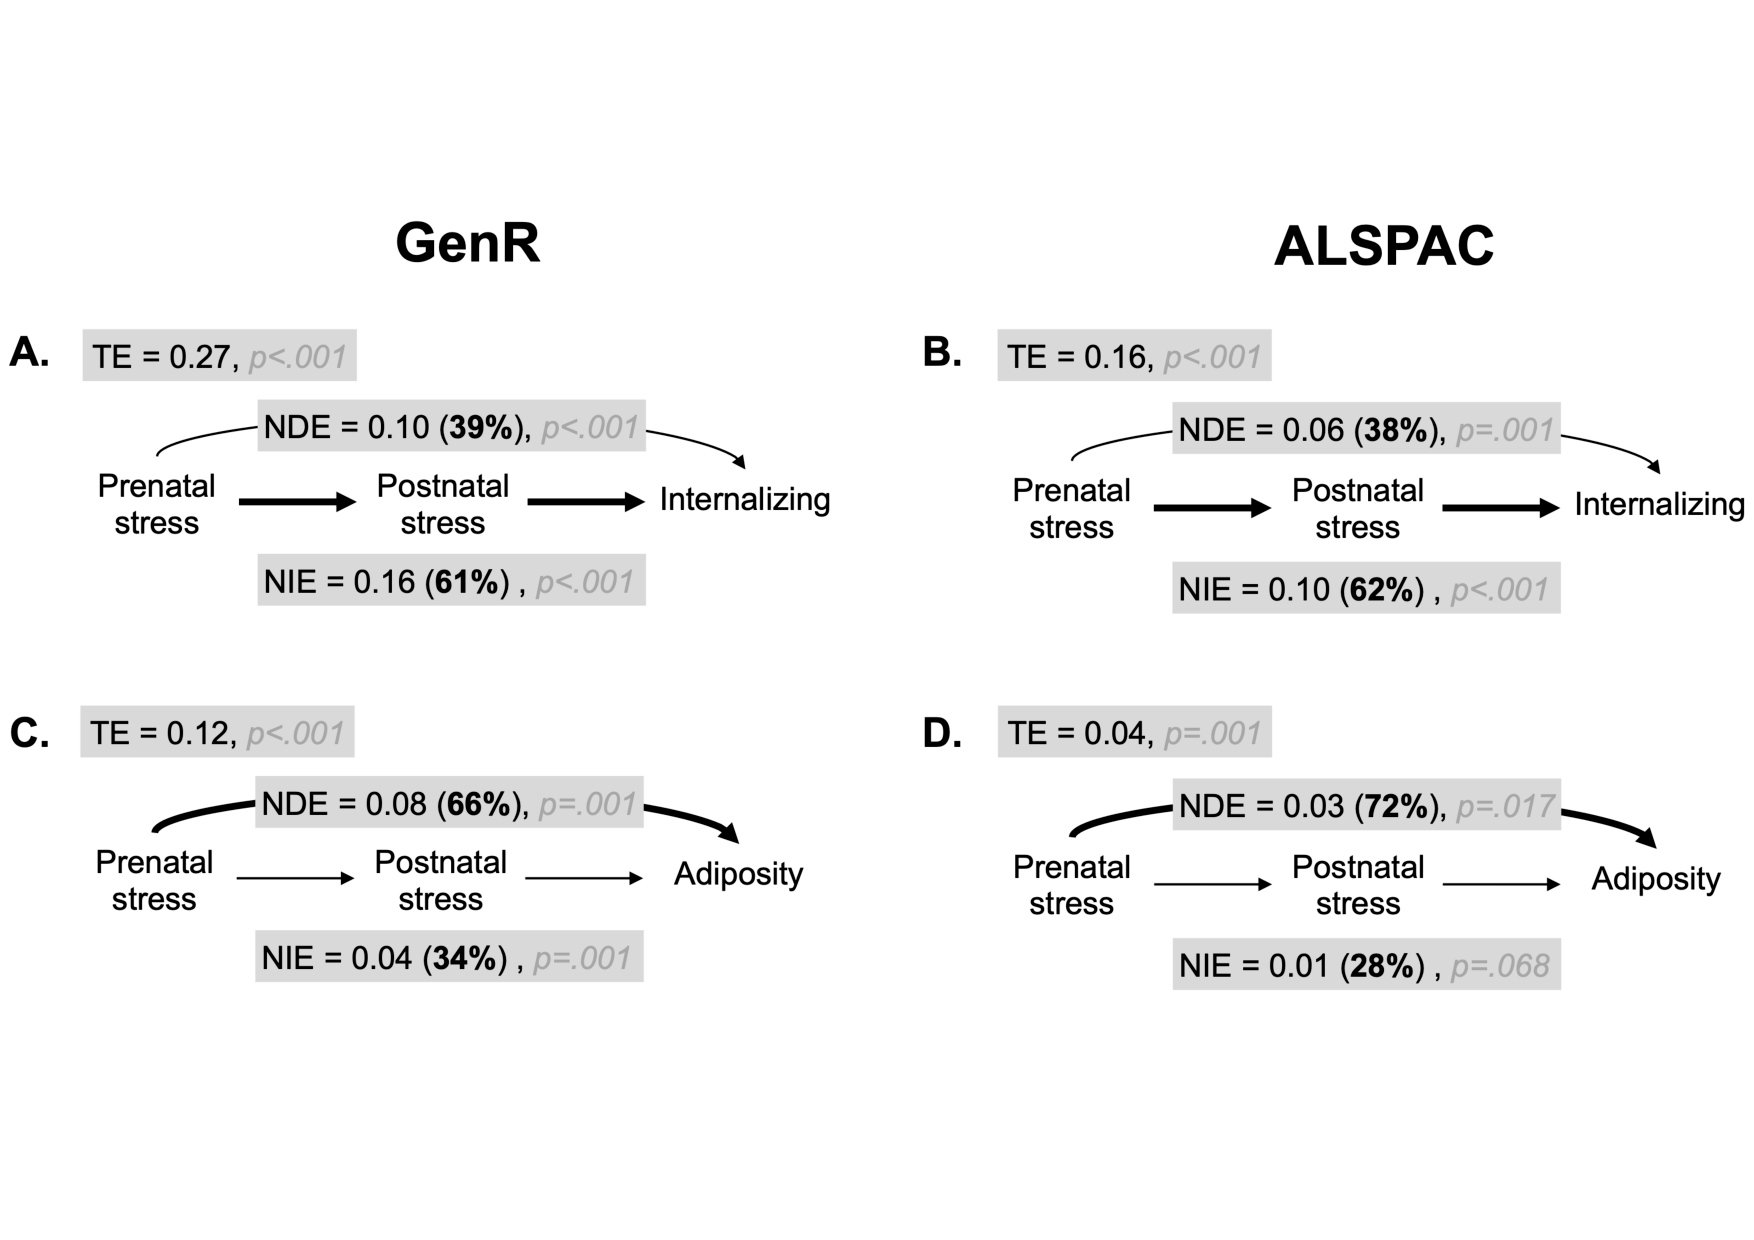
\includegraphics[width=1\linewidth,height=\textheight,keepaspectratio]{2.Chapter/Figures/F2_CMAres.pdf}

}

\caption{\label{fig-2.2}\textbf{Prenatal early-life stress (ELS)
contribution (causal mediation analysis results)}\newline(A-D) The
causal estimates for the total effect (TE), natural direct (NDE) and
natural indirect effect (NIE) of prenatal stress on internalizing
symptoms (A. Generation R and B. ALSPAC) and adiposity (C. Generation R
and D. ALSPAC) are displayed in the grey boxes. The percentage of the
total effect due to direct and indirect pathway is reported between
brackets and the respective p-values are marked in grey. The predominant
path is highlighted with a thicker arrow. NDE = natural direct effect;
NIE = natural indirect effect; TE = total effect.}

\end{figure}%

\subsection{Association of postnatal ELS with internalizing symptoms and
adiposity}\label{association-of-postnatal-els-with-internalizing-symptoms-and-adiposity-1}

Results of the hierarchical regressions examining the association of
postnatal stress with internalizing and adiposity were also largely
similar across cohorts (see Figure~\ref{fig-2.3}; online
\href{https://osf.io/7e4x8}{\emph{Tables S3 and S4}}).

Higher postnatal stress associated with increased internalizing symptoms
both before (\(\beta\) {[}95\%CI{]} = GenR: 0.33 {[}0.29;0.37{]};
ALSPAC: 0.22 {[}0.19;0.25{]}) and after adjustment for prenatal stress
(GenR: 0.27 {[}0.22;0.31{]}; ALSPAC: 0.19 {[}0.15;0.22{]}).

Higher postnatal stress also associated with increased adiposity (GenR:
0.10 {[}0.07;0.13{]}; ALSPAC: 0.03 {[}0.01;0.05{]}). The association
remained after prenatal stress adjustment in GenR (0.07
{[}0.03;0.11{]}), but not in ALSPAC (0.02 {[}0.00;0.05{]}).

\begin{figure}[H]

\centering{

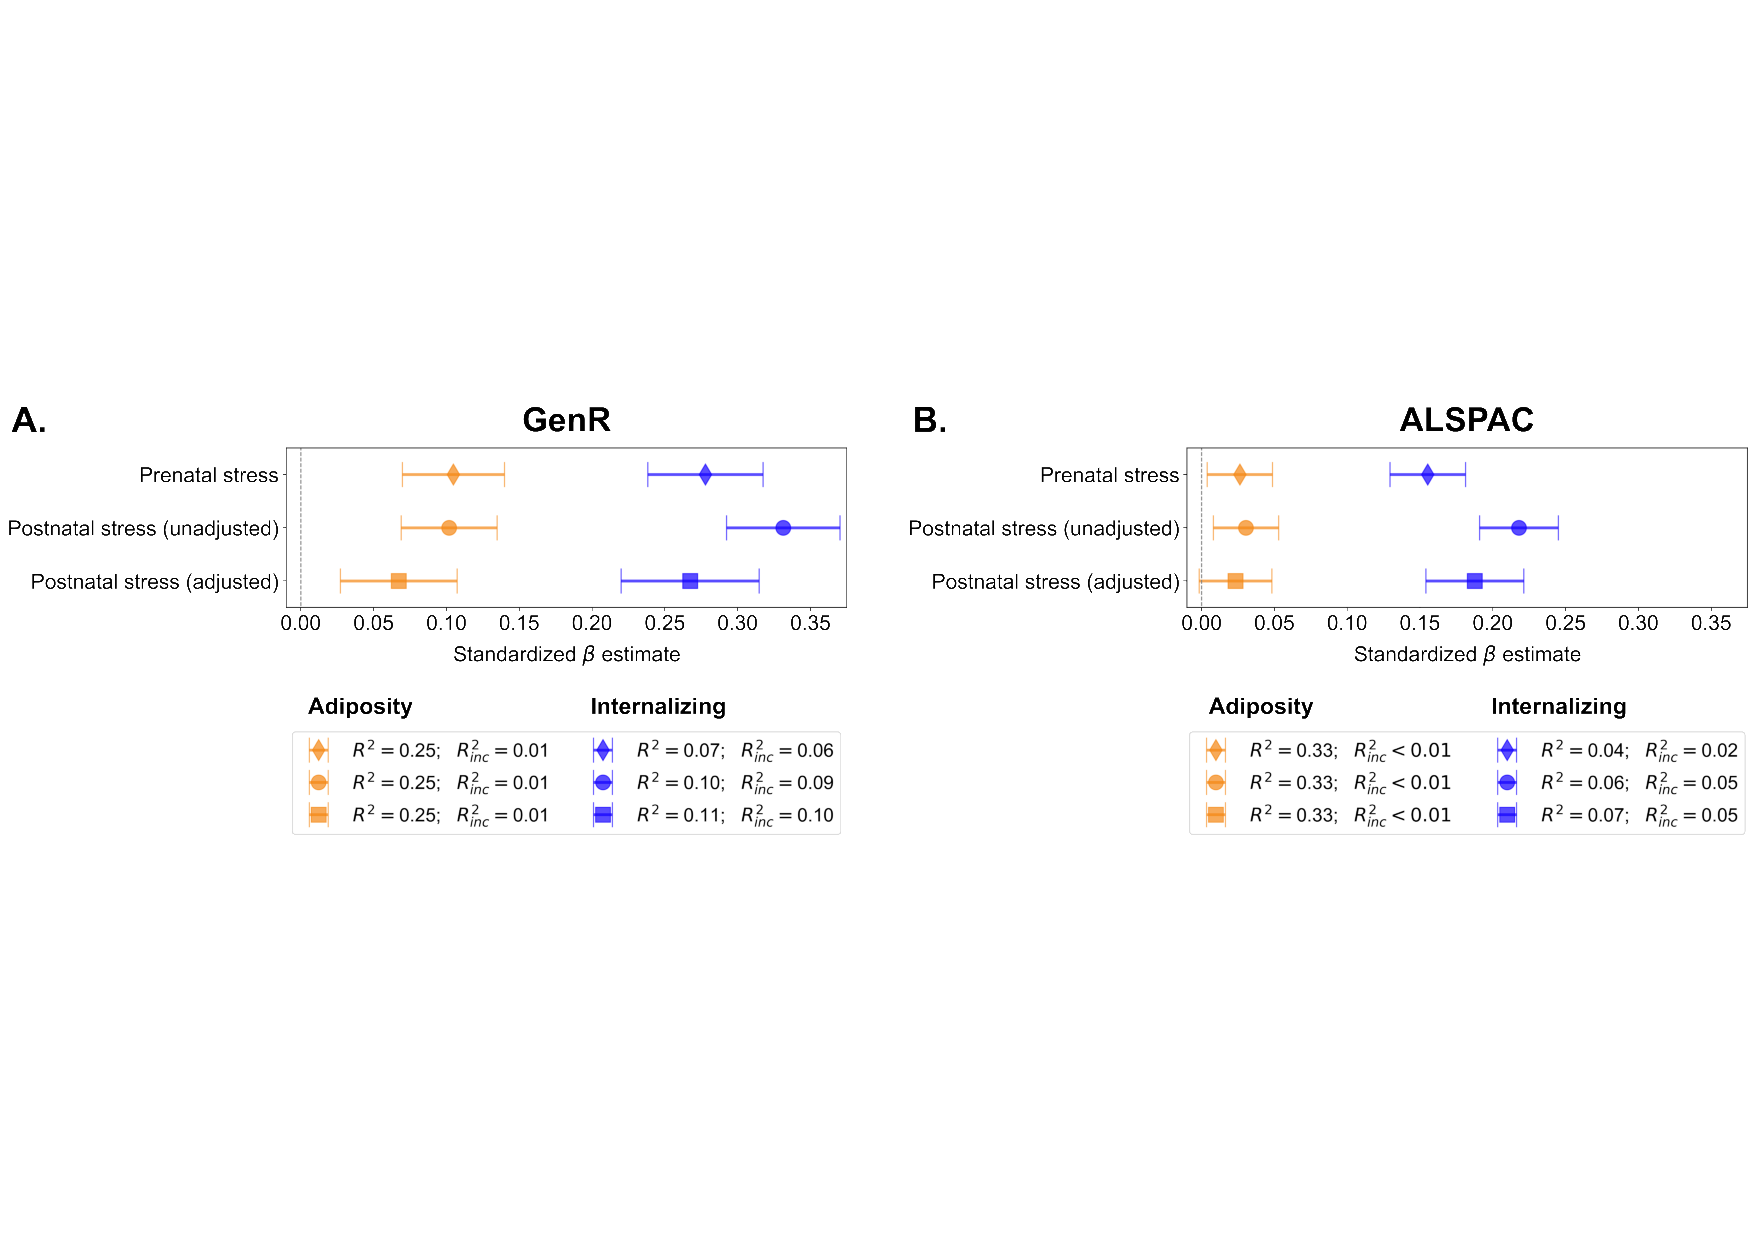
\includegraphics[width=1\linewidth,height=\textheight,keepaspectratio]{2.Chapter/Figures/F3_regress.pdf}

}

\caption{\label{fig-2.3}\textbf{Postnatal early-life stress (ELS)
contribution (hierarchical regression results)}\newline(A, B) In each
cohort (A. Generation R and B. ALSPAC), the standardized beta estimates
of pre- and postnatal ELS (and their 95\% confidence intervals) are
represented along the x-axis, using different color sets for
internalizing symptoms (light and dark blue) and adiposity (yellow and
orange). Estimates generated by the prenatal only model are presented on
the first row and marked in lighter colours (i.e., light blue and
yellow); these correspond to the TE displayed in Figure 2. Postnatal ELS
beta estimates, before (round marker) and after (square marker) prenatal
adjustment, are displayed in darker colors (blue and orange). For each
model, the total and incremental R2 is reported in the legend below the
graphs. The first number provides an indication of total model fit; the
latter quantifies the increase in variance explained due to the
introduction of the predictor (compared to the covariate only model).}

\end{figure}%

\subsection{Association of prenatal and postnatal ELS with
comorbidity}\label{association-of-prenatal-and-postnatal-els-with-comorbidity-1}

Higher stress in the prenatal (OR {[}95\%CI{]} = GenR: 2.13
{[}1.84;2.47{]}; ALSPAC: 1.48 {[}1.28;1.71{]}) and postnatal periods
(GenR: 2.37 {[}2.05;2.75{]}; ALSPAC: 1.61 {[}1.39;1.87{]}) was
associated with higher odds of belonging to the comorbidity group
compared to the healthy group (see Figure~\ref{fig-2.4} and online
\href{https://osf.io/7e4x8}{\emph{Table S5}}). This association was the
strongest compared to all other (single-outcome) groups. However, the
CIs of the comorbidity estimates did overlap with those of high
internalizing only (Figure~\ref{fig-2.4} C and D).

\begin{figure}[H]

\centering{

\includegraphics[width=1\linewidth,height=\textheight,keepaspectratio]{2.Chapter/Figures/F4_comorb.pdf}

}

\caption{\label{fig-2.4}\textbf{Pre- and postnatal early-life stress
(ELS) and psycho-cardiometabolic comorbidity}\newline(A, B) Scatterplots
of internalizing symptoms (on the x axis) and fat mass percentage (on
the y-axis), for the Generation R (A) and ALSPAC (B) cohorts. The
univariate distributions of both primary outcomes are shown on the
respective axes, with darker shadow indicating the 80th percentile
cut-off used in construction of the comorbidity variable. Colour
indicates the assigned group (green = healthy; blue = high
internalizing; yellow = high adiposity; red = comorbid). Group sizes
(i.e., n and percent of the total cohort sample) were pooled across
imputed datasets and reported on the right of each
scatterplot.\newline(C, D) Effect estimates for pre- and postnatal
stress (and their 95\%CIs) on the odds ratio (OR) scale are represented
along the x-axis, with different colours depending on the comparison
they refer to (yellow = healthy vs.~high adiposity; blue = healthy
vs.~high internalizing; red = healthy vs.~comorbid), in Generation R (C)
and ALSPAC (D) children.}

\end{figure}%

\subsection{Follow-up analyses}\label{follow-up-analyses}

\subsubsection{Interaction with sex and ethnic
background}\label{interaction-with-sex-and-ethnic-background}

After stratifying by sex, in GenR, the association between prenatal ELS
and adiposity was larger in girls than in boys (\emph{Z}=1.89,
\emph{p}=.029), whereas that of postnatal ELS was slightly larger in
boys (\emph{Z}=-1.38, \emph{p}=.083). A similar pattern of associations
was found in ALSPAC but with smaller magnitudes (see
\href{https://osf.io/xs29c}{\emph{Figures S2-S4}} and
\href{https://osf.io/7e4x8}{\emph{Tables S6-S9}}, available online).

In GenR, Cape Verdian and Dutch Antillean children experienced the
highest cumulative prenatal and postnatal stress followed by Turkish,
Surinamese and Moroccan children
(\href{https://osf.io/xs29c}{\emph{Figure S5-B}}). We did not find
evidence for a significant interaction between pre- or postnatal ELS and
the examined ethnic background groups on any outcome of interest (i.e.,
internalizing symptoms, adiposity or comorbidity; see
\href{https://osf.io/7e4x8}{\emph{Table S10}} and
\href{https://osf.io/xs29c}{\emph{Figure S5-C}}, available online). Note
however that the association between pre-/postnatal ELS and comorbidity
in the ``North American'' group could not be estimated due to
insufficient number of observations (i.e., comorbidity group size ≤ 5).

\subsubsection{Contribution of specific stress
domains}\label{contribution-of-specific-stress-domains}

Across cohorts, internalizing symptoms were consistently associated with
higher prenatal and postnatal parental risk (e.g., parental
psychopathology), postnatal life events and direct victimization (see
\href{https://osf.io/xs29c}{\emph{Figure S6}} and
\href{https://osf.io/7e4x8}{\emph{Table S11}}, available online). We
found no consistent associations for adiposity. Only postnatal parental
risk was consistently associated comorbidity status (vs.~healthy) across
cohorts (see \href{https://osf.io/xs29c}{\emph{Figure S7}} and
\href{https://osf.io/7e4x8}{\emph{Table S12}}, available online).

\subsubsection{Sensitivity analyses}\label{sensitivity-analyses}

Restricting the analyses to participants with complete outcome data (n =
GenR: 2749; ALSPAC: 4096) did not substantively change the reported
findings (see \href{https://osf.io/xs29c}{\emph{Figure S8}} and
\href{https://osf.io/7e4x8}{\emph{Tables S13-S15}}, available online),
nor did the use of android fat mass rather than fat mass percentage as a
proxy of adiposity (see \href{https://osf.io/xs29c}{\emph{Figure S9}}
and \href{https://osf.io/7e4x8}{\emph{Table S16}}, available online).
None of the main conclusions was impacted by FDR correction.

\section{Discussion}\label{discussion}

Our aim was to elucidate the role of ELS on adolescent internalizing
problems and adiposity, as well as their comorbidity, based on
prospective data from two population birth cohorts. We highlight two key
findings. Firstly, exposure to cumulative stress is strongly associated
with internalizing symptoms (especially postnatal ELS) and, to a lesser
extent, with adiposity (especially prenatal ELS). Secondly, both pre-
and postnatal stress associate with psycho-cardiometabolic comorbidity
more strongly than to individual health outcomes.

Our first objective was to disentangle the relative contribution of
prenatal and postnatal stress exposure to adolescent internalizing
symptoms and adiposity.

We found that, although both pre- and postnatal ELS contribute to
internalizing symptoms, the impact of postnatal stress is larger and it
is not explained by prenatal confounding, while \textasciitilde60\% of
the prenatal effect was mediated though postnatal stress. This finding
aligns with previous studies investigating the contribution of prenatal
and postnatal exposure to specific stressors (Clayborne et al., 2021;
Plant et al., 2015), and holds promising clinical implications given
that several aspects of the postnatal environment may be modifiable (Yap
et al., 2016). In particular, parental risk factors (such as
psychopathology), direct victimization (e.g., maltreatment) and life
events emerged as independent predictors of internalizing symptoms in
our exploratory analyses, indicating that these may represent important
targets for intervention.

To our knowledge, no study to date has explored such timing effects on
adiposity or related outcomes. Here, we found that \textasciitilde70\%
of the effect of prenatal stress on adiposity was ``direct'' (i.e., not
mediated by postnatal stress); the effect of postnatal stress, both as
mediator and as predictor in the adjusted models, was smaller and
resulted statistically significant only in GenR. While it is important
to note that the effect sizes observed in the adiposity models were
markedly smaller than for internalizing symptoms, these findings provide
some indication that fat accumulation processes could be particularly
vulnerable to (stress-induced) alterations of the prenatal environment.
This is in line with previous theoretical (Barker, 1998; Gluckman et
al., 2008) and empirical (Entringer et al., 2012; Entringer, 2013)
accounts showcasing the impact of stress and stress hormones during
prenatal life on the programming of metabolic function and obesity risk.
In our exploratory follow-up analyses, we additionally found some
evidence that adiposity may be more strongly associated with prenatal
stress in girls, versus postnatal stress in boys. However previous
accounts of these sex differences are mixed (Murphy \& Loria, 2017;
Paternain et al., 2013), and differences in pubertal development may be
an important confounding factor that was not accounted for in our
analysis.

It is also possible that stronger associations between postnatal ELS and
adiposity will emerge later in development. Indeed, accumulating
postnatal risks may influence biological (e.g., inflammatory and
neuro-endocrine) and behavioral factors (e.g., diet and exercise) that
in turn increase physical health burden, but this might become evident
only later in life (Danese \& Tan, 2014; Elsenburg et al., 2017).

Our second aim was to examine whether ELS relates to
psycho-cardiometabolic comorbidity, as suggested by some theoretical
accounts (Juster et al., 2016), but never explicitly investigated
before. If comorbidity was a discrete stress-related pathophysiological
process, then the effect of ELS on comorbidity would differ from the
effect of ELS on mental and physical health separately. This expectation
was partially confirmed by our data: ELS increased the risk of
developing comorbidity compared to being healthy and this estimate was
highest relative to all other groups. However, the overlap between CIs
of the comorbidity and the internalizing-only estimate indicates that
neither pre- nor postnatal stress levels were sufficient to predict
whether a child will develop comorbidity vs.~internalizing problems
alone. Notably, cross-sectional correlations between internalizing and
adiposity at age 13 were small (and so were the comorbidity group
sizes), which may partly explain these findings. However, comorbidity is
known to increase with age (Barnett et al., 2012) and it is possible
that pre- / postnatal stress may serve as better discriminators between
comorbidity and internalizing problems in older samples, with higher
comorbidity rates.

This study has several important strengths. We analysed data from two
large population-based cohorts with remarkably consistent results, which
adds confidence to the robustness and generalizability of our findings.
We used a longitudinal and comprehensive assessment of ELS, enabling us
to quantify the relative contribution of pre- and postnatal exposure to
a broad spectrum of stressors. We focused on two pre-clinical health
markers which manifest in adolescence and may be important targets for
early prevention. Also, the challenge of incomplete data and possible
selection bias was thoroughly addressed by multiple imputation and
sensitivity analyses. However, it is important to note that our measures
of ELS and internalizing symptoms rely primarily on parent reports,
which might have introduced information bias. Further, although several
important confounders were taken into account, it will be important in
the future to examine the role of other potential contributors,
including (epi-)genetic influences (Inoue et al., 2022), pubertal
status, disability/functional impairment and other behavioral factors
(e.g., sleep, exercise, diet).

In conclusion, current approaches to the prevention and management of
depression and obesity have yielded limited success. We believe the
adoption of an integrated, developmental framework is necessary to
improve our understanding and set the stage for better detection and
prevention of these disorders, both in isolation and in their comorbid
form. We provide evidence that both pre- and postnatal ELS associate
with adolescent internalizing symptoms (with prenatal \textless{}
postnatal stress), adiposity (with prenatal \textgreater{} postnatal
stress), and their comorbidity at age 13. While recommendations for how
to best intervene when a higher psychosocial stress burden is identified
are still at embryonic stage, one novel suggestion emerging from our
findings is that prenatal stress may be an underrecognized factor for
identifying children at higher risk of overweight. We would therefore
advice clinicians to enquire about prenatal stress exposure as part of
routine pediatric assessments, so that adequate monitoring and lifestyle
preventative measures can be introduced as early as infancy.

Finally, as we follow these children, it will be informative to see how
these associations evolve over time. For instance, the association
between ELS exposure and adiposity-related outcomes may not emerge fully
until adulthood and it is possible that the nature of the relation
between ELS and comorbidity also differs as a function of developmental
stage.

\section*{References}\label{references-1}
\addcontentsline{toc}{section}{References}

\markright{References}

\phantomsection\label{refs--2}
\begin{CSLReferences}{1}{0}
\bibitem[\citeproctext]{ref-Achenbach1999}
Achenbach, T. M. (1999). The child behavior checklist and related
instruments {[}Book Section{]}. In \emph{The use of psychological
testing for treatment planning and outcomes assessment, 2nd ed.} (pp.
429--466). Lawrence Erlbaum Associates Publishers.

\bibitem[\citeproctext]{ref-Alders2001}
Alders, M. (2001). \emph{Classification of the population with a foreign
background in the netherlands} {[}Journal Article{]}.

\bibitem[\citeproctext]{ref-Anwar2018}
Anwar, N., Kuppili, P. P., \& Balhara, Y. P. S. (2018). Depression and
physical noncommunicable diseases: The need for an integrated approach
{[}Journal Article{]}. \emph{WHO South-East Asia Journal of Public
Health}, \emph{6}(1), 12--17.

\bibitem[\citeproctext]{ref-Barker1998}
Barker, D. J. (1998). In utero programming of chronic disease {[}Journal
Article{]}. \emph{Clinical Science (London, England: 1979)},
\emph{95}(2), 115--128.

\bibitem[\citeproctext]{ref-Barnett2012}
Barnett, K., Mercer, S. W., Norbury, M., Watt, G., Wyke, S., \& Guthrie,
B. (2012). Epidemiology of multimorbidity and implications for health
care, research, and medical education: A cross-sectional study
{[}Journal Article{]}. \emph{The Lancet}, \emph{380}(9836), 37--43.
\url{https://doi.org/10.1016/S0140-6736(12)60240-2}

\bibitem[\citeproctext]{ref-Boyd2013}
Boyd, A., Golding, J., Macleod, J., Lawlor, D. A., Fraser, A.,
Henderson, J., Molloy, L., Ness, A., Ring, S., \& Davey Smith, G.
(2013). Cohort profile: The 'children of the 90s'---the index offspring
of the avon longitudinal study of parents and children {[}Journal
Article{]}. \emph{International Journal of Epidemiology}, \emph{42}(1),
111--127. \url{https://doi.org/10.1093/ije/dys064}

\bibitem[\citeproctext]{ref-Burgueuxf1o2020}
Burgueño, A. L., Juarez, Y. R., Genaro, A. M., \& Tellechea, M. L.
(2020). Systematic review and meta-analysis on the relationship between
prenatal stress and metabolic syndrome intermediate phenotypes
{[}Journal Article{]}. \emph{International Journal of Obesity},
\emph{44}(1), 1--12. \url{https://doi.org/10.1038/s41366-019-0423-z}

\bibitem[\citeproctext]{ref-Cecil2014}
Cecil, C. A., Lysenko, L. J., Jaffee, S. R., Pingault, J. B., Smith, R.
G., Relton, C. L., Woodward, G., McArdle, W., Mill, J., \& Barker, E. D.
(2014). Environmental risk, oxytocin receptor gene (OXTR) methylation
and youth callous-unemotional traits: A 13-year longitudinal study
{[}Journal Article{]}. \emph{Mol Psychiatry}, \emph{19}(10), 1071--1077.
\url{https://doi.org/10.1038/mp.2014.95}

\bibitem[\citeproctext]{ref-Cecil2017}
Cecil, C. A., Viding, E., Fearon, P., Glaser, D., \& McCrory, E. J.
(2017). Disentangling the mental health impact of childhood abuse and
neglect {[}Journal Article{]}. \emph{Child Abuse \& Neglect}, \emph{63},
106--119. \url{https://doi.org/10.1016/j.chiabu.2016.11.024}

\bibitem[\citeproctext]{ref-Clayborne2021}
Clayborne, Z. M., Nilsen, W., Torvik, F. A., Gustavson, K., Bekkhus, M.,
Gilman, S. E., Khandaker, G. M., Fell, D. B., \& Colman, I. (2021).
Prenatal maternal stress, child internalizing and externalizing
symptoms, and the moderating role of parenting: Findings from the
norwegian mother, father, and child cohort study {[}Journal Article{]}.
\emph{Psychological Medicine}, 1--11.
\url{https://doi.org/10.1017/S0033291721004311}

\bibitem[\citeproctext]{ref-Danese2014}
Danese, A., \& Tan, M. (2014). Childhood maltreatment and obesity:
Systematic review and meta-analysis {[}Journal Article{]}. \emph{Mol
Psychiatry}, \emph{19}(5), 544--554.
\url{https://doi.org/10.1038/mp.2013.54}

\bibitem[\citeproctext]{ref-vonElm2008}
Elm, E. von, Altman, D. G., Egger, M., Pocock, S. J., Gøtzsche, P. C.,
\& Vandenbroucke, J. P. (2008). The strengthening the reporting of
observational studies in epidemiology (STROBE) statement: Guidelines for
reporting observational studies {[}Journal Article{]}. \emph{J Clin
Epidemiol}, \emph{61}(4), 344--349.
\url{https://doi.org/10.1016/j.jclinepi.2007.11.008}

\bibitem[\citeproctext]{ref-Elsenburg2017}
Elsenburg, L. K., Wijk, K. J. E. van, Liefbroer, A. C., \& Smidt, N.
(2017). Accumulation of adverse childhood events and overweight in
children: A systematic review and meta-analysis {[}Journal Article{]}.
\emph{Obesity (Silver Spring)}, \emph{25}(5), 820--832.
\url{https://doi.org/10.1002/oby.21797}

\bibitem[\citeproctext]{ref-Entringer2013}
Entringer, S. (2013). Impact of stress and stress physiology during
pregnancy on child metabolic function and obesity risk {[}Journal
Article{]}. \emph{Current Opinion in Clinical Nutrition and Metabolic
Care}, \emph{16}(3), 320--327.
\url{https://doi.org/10.1097/MCO.0b013e32835e8d80}

\bibitem[\citeproctext]{ref-Entringer2012}
Entringer, S., Buss, C., Swanson, J. M., Cooper, D. M., Wing, D. A.,
Waffarn, F., \& Wadhwa, P. D. (2012). Fetal programming of body
composition, obesity, and metabolic function: The role of intrauterine
stress and stress biology {[}Journal Article{]}. \emph{J Nutr Metab},
\emph{2012}, 632548. \url{https://doi.org/10.1155/2012/632548}

\bibitem[\citeproctext]{ref-Fraser2013}
Fraser, A., Macdonald-Wallis, C., Tilling, K., Boyd, A., Golding, J.,
Davey Smith, G., Henderson, J., Macleod, J., Molloy, L., Ness, A., Ring,
S., Nelson, S. M., \& Lawlor, D. A. (2013). Cohort profile: The avon
longitudinal study of parents and children: ALSPAC mothers cohort
{[}Journal Article{]}. \emph{Int J Epidemiol}, \emph{42}(1), 97--110.
\url{https://doi.org/10.1093/ije/dys066}

\bibitem[\citeproctext]{ref-Gluckman2008}
Gluckman, P. D., Hanson, M. A., Cooper, C., \& Thornburg, K. L. (2008).
Effect of in utero and early-life conditions on adult health and disease
{[}Journal Article{]}. \emph{New England Journal of Medicine},
\emph{359}(1), 61--73.

\bibitem[\citeproctext]{ref-Goodman2000}
Goodman, R., Ford, T., Richards, H., Gatward, R., \& Meltzer, H. (2000).
The development and well-being assessment: Description and initial
validation of an integrated assessment of child and adolescent
psychopathology {[}Journal Article{]}. \emph{J Child Psychol
Psychiatry}, \emph{41}(5), 645--655.

\bibitem[\citeproctext]{ref-Goodman1999}
Goodman, R., \& Scott, S. (1999). Comparing the strengths and
difficulties questionnaire and the child behavior checklist: Is small
beautiful? {[}Journal Article{]}. \emph{Journal of Abnormal Child
Psychology}, \emph{27}(1), 17--24.
\url{https://doi.org/10.1023/A:1022658222914}

\bibitem[\citeproctext]{ref-Hare2014}
Hare, D. L., Toukhsati, S. R., Johansson, P., \& Jaarsma, T. (2014).
Depression and cardiovascular disease: A clinical review {[}Journal
Article{]}. \emph{Eur Heart J}, \emph{35}(21), 1365--1372.
\url{https://doi.org/10.1093/eurheartj/eht462}

\bibitem[\citeproctext]{ref-Hartman2018}
Hartman, S., \& Belsky, J. (2018). Prenatal programming of postnatal
plasticity revisited-and extended {[}Journal Article{]}. \emph{Dev
Psychopathol}, \emph{30}(3), 825--842.
\url{https://doi.org/10.1017/s0954579418000548}

\bibitem[\citeproctext]{ref-Inoue2022}
Inoue, Y., Graff, M., Howard, A. G., Highland, H. M., Young, K. L.,
Harris, K. M., North, K. E., Li, Y., Duan, Q., \& Gordon-Larsen, P.
(2022). Do adverse childhood experiences and genetic obesity risk
interact in relation to body mass index in young adulthood? Findings
from the national longitudinal study of adolescent to adult health
{[}Journal Article{]}. \emph{Pediatr Obes}, \emph{17}(6), e12885.
\url{https://doi.org/10.1111/ijpo.12885}

\bibitem[\citeproctext]{ref-Juster2016}
Juster, R. P., Russell, J. J., Almeida, D., \& Picard, M. (2016).
Allostatic load and comorbidities: A mitochondrial, epigenetic, and
evolutionary perspective {[}Journal Article{]}. \emph{Dev Psychopathol},
\emph{28}(4pt1), 1117--1146.
\url{https://doi.org/10.1017/s0954579416000730}

\bibitem[\citeproctext]{ref-Kooijman2016}
Kooijman, M. N., Kruithof, C. J., Duijn, C. M. van, Duijts, L., Franco,
O. H., Ijzendoorn, M. H. van, Jongste, J. C. de, Klaver, C. C. W., Lugt,
A. van der, Mackenbach, J. P., Moll, H. A., Peeters, R. P., Raat, H.,
Rings, E. H. H. M., Rivadeneira, F., Schroeff, M. P. van der, Steegers,
E. A. P., Tiemeier, H., Uitterlinden, A. G., \ldots{} Jaddoe, V. W. V.
(2016). The generation r study: Design and cohort update 2017 {[}Journal
Article{]}. \emph{European Journal of Epidemiology}, \emph{31}(12),
1243--1264. \url{https://doi.org/10.1007/s10654-016-0224-9}

\bibitem[\citeproctext]{ref-Li2016}
Li, M., D'Arcy, C., \& Meng, X. (2016). Maltreatment in childhood
substantially increases the risk of adult depression and anxiety in
prospective cohort studies: Systematic review, meta-analysis, and
proportional attributable fractions {[}Journal Article{]}. \emph{Psychol
Med}, \emph{46}(4), 717--730.
\url{https://doi.org/10.1017/s0033291715002743}

\bibitem[\citeproctext]{ref-Murphy2017}
Murphy, M. O., \& Loria, A. S. (2017). Sex-specific effects of stress on
metabolic and cardiovascular disease: Are women at higher risk?
{[}Journal Article{]}. \emph{American Journal of Physiology-Regulatory,
Integrative and Comparative Physiology}, \emph{313}(1), R1--R9.
\url{https://doi.org/10.1152/ajpregu.00185.2016}

\bibitem[\citeproctext]{ref-Paternain2013}
Paternain, L., De La Garza, A., Batlle, M., Milagro, F., Martinez, J.
A., \& Campion, J. (2013). Prenatal stress increases the obesogenic
effects of a high-fat-sucrose diet in adult rats in a sex-specific
manner {[}Journal Article{]}. \emph{Stress}, \emph{16}(2), 220--232.

\bibitem[\citeproctext]{ref-Pereira-Miranda2017}
Pereira-Miranda, E., Costa, P. R. F., Queiroz, V. A. O., Pereira-Santos,
M., Santana, M. L. P., \& Santana, M. L. P. (2017). Overweight and
obesity associated with higher depression prevalence in adults: A
systematic review and meta-analysis {[}Journal Article{]}. \emph{J Am
Coll Nutr}, \emph{36}(3), 223--233.
\url{https://doi.org/10.1080/07315724.2016.1261053}

\bibitem[\citeproctext]{ref-Plant2015}
Plant, D. T., Pariante, C. M., Sharp, D., \& Pawlby, S. (2015). Maternal
depression during pregnancy and offspring depression in adulthood: Role
of child maltreatment {[}Journal Article{]}. \emph{Br J Psychiatry},
\emph{207}(3), 213--220. \url{https://doi.org/10.1192/bjp.bp.114.156620}

\bibitem[\citeproctext]{ref-Pratt2014}
Pratt, L. A., \& Brody, D. J. (2014). Depression and obesity in the u.s.
Adult household population, 2005-2010 {[}Journal Article{]}. \emph{NCHS
Data Brief}, \emph{167}, 1--8.

\bibitem[\citeproctext]{ref-R2021}
R Core Team. (2021). \emph{R: A language and environment for statistical
computing} {[}Journal Article{]}. \url{https://www.R-project.org/}

\bibitem[\citeproctext]{ref-Rijlaarsdam2016}
Rijlaarsdam, J., Pappa, I., Walton, E., Bakermans-Kranenburg, M. J.,
Mileva-Seitz, V. R., Rippe, R. C., Roza, S. J., Jaddoe, V. W., Verhulst,
F. C., Felix, J. F., Cecil, C. A., Relton, C. L., Gaunt, T. R., McArdle,
W., Mill, J., Barker, E. D., Tiemeier, H., \& van, Ij. M. H. (2016). An
epigenome-wide association meta-analysis of prenatal maternal stress in
neonates: A model approach for replication {[}Journal Article{]}.
\emph{Epigenetics}, \emph{11}(2), 140--149.
\url{https://doi.org/10.1080/15592294.2016.1145329}

\bibitem[\citeproctext]{ref-Schuurmans2022}
Schuurmans, I. K., Luik, A. I., Maat, D. A. de, Hillegers, M. H. J.,
Ikram, M. A., \& Cecil, C. A. M. (2022). The association of early life
stress with IQ-achievement discrepancy in children: A population-based
study {[}Journal Article{]}. \emph{Child Development}, \emph{93}(6),
1837--1847. \url{https://doi.org/10.1111/cdev.13825}

\bibitem[\citeproctext]{ref-Shonkoff2012}
Shonkoff, J. P., Garner, A. S., Siegel, B. S., Dobbins, M. I., Earls, M.
F., Garner, A. S., McGuinn, L., Pascoe, J., \& Wood, D. L. (2012). The
lifelong effects of early childhood adversity and toxic stress
{[}Journal Article{]}. \emph{Pediatrics}, \emph{129}(1), e232--e246.
\url{https://doi.org/10.1542/peds.2011-2663}

\bibitem[\citeproctext]{ref-Slopen2014}
Slopen, N., Koenen, K. C., \& Kubzansky, L. D. (2014). Cumulative
adversity in childhood and emergent risk factors for long-term health
{[}Journal Article{]}. \emph{J Pediatr}, \emph{164}(3), 631-8.e1-2.
\url{https://doi.org/10.1016/j.jpeds.2013.11.003}

\bibitem[\citeproctext]{ref-Sutaria2019}
Sutaria, S., Devakumar, D., Yasuda, S. S., Das, S., \& Saxena, S.
(2019). Is obesity associated with depression in children? Systematic
review and meta-analysis {[}Journal Article{]}. \emph{Archives of
Disease in Childhood}, \emph{104}(1), 64--74.
\url{https://doi.org/10.1136/archdischild-2017-314608}

\bibitem[\citeproctext]{ref-vanBuuren2018}
Van Buuren, S. (2018). \emph{Flexible imputation of missing data} (2nd
ed.). Chapman; Hall/CRC. \url{https://doi.org/10.1201/9780429492259}

\bibitem[\citeproctext]{ref-VandenBergh2020}
Van den Bergh, B. R. H., Heuvel, M. I. van den, Lahti, M., Braeken, M.,
Rooij, S. R. de, Entringer, S., Hoyer, D., Roseboom, T., Räikkönen, K.,
King, S., \& Schwab, M. (2020). Prenatal developmental origins of
behavior and mental health: The influence of maternal stress in
pregnancy {[}Journal Article{]}. \emph{Neurosci Biobehav Rev},
\emph{117}, 26--64.
\url{https://doi.org/10.1016/j.neubiorev.2017.07.003}

\bibitem[\citeproctext]{ref-Voortman2016}
Voortman, T., Leermakers, E. T. M., Franco, O. H., Jaddoe, V. W. V.,
Moll, H. A., Hofman, A., Hooven, E. H. van den, \& Kiefte-de Jong, J. C.
(2016). A priori and a posteriori dietary patterns at the age of 1~year
and body composition at the age of 6~years: The generation r study
{[}Journal Article{]}. \emph{European Journal of Epidemiology},
\emph{31}(8), 775--783. \url{https://doi.org/10.1007/s10654-016-0179-x}

\bibitem[\citeproctext]{ref-Wang2015}
Wang, A., \& Arah, O. A. (2015). G-computation demonstration in causal
mediation analysis {[}Journal Article{]}. \emph{Eur J Epidemiol},
\emph{30}(10), 1119--1127.
\url{https://doi.org/10.1007/s10654-015-0100-z}

\bibitem[\citeproctext]{ref-Yap2016}
Yap, M. B. H., Morgan, A. J., Cairns, K., Jorm, A. F., Hetrick, S. E.,
\& Merry, S. (2016). Parents in prevention: A meta-analysis of
randomized controlled trials of parenting interventions to prevent
internalizing problems in children from birth to age 18 {[}Journal
Article{]}. \emph{Clinical Psychology Review}, \emph{50}, 138--158.
\url{https://doi.org/10.1016/j.cpr.2016.10.003}

\end{CSLReferences}

\chapter{Lifestyle factors, ELS and adolescent psycho-physical
health}\label{sec-chapter3}

Adapted from:

\textbf{The role of lifestyle factors in the association between
early-life stress and adolescent psycho-physical health: Moderation
analysis in two European birth cohorts}

\textbf{Defina, S.}, Woofenden, T., Baltramonaityte, V., Tiemeier, H.,
Fairchild, G., Felix, J. F., Cecil, C.A.M., \& Walton, E. (2024).
\emph{Preventive Medicine}.
\href{https://doi.org/10.1016/j.ypmed.2024.107926}{DOI}

\section*{Abstract}\label{abstract-1}
\addcontentsline{toc}{section}{Abstract}

\markright{Abstract}

\ul{Objective}: Early-life stress (ELS) is an established risk factor
for a host of adult mental and physical health problems, including both
depression and obesity. Recent studies additionally showed that ELS was
associated with an increased risk of comorbidity between mental and
physical health problems, already in adolescence. Healthy lifestyle
factors, including physical activity, sleep and diet have also been
robustly linked to both emotional and physical wellbeing. However, it is
yet unclear whether these lifestyle factors may moderate the association
between ELS and psycho-physical comorbidity.

\ul{Methods}: We investigated whether \emph{(a)} participation in
physical activity, \emph{(b)} sleep duration, and \emph{(c)} adherence
to a Mediterranean diet, moderated the relationship between cumulative
ELS exposure over the first 10 years of life and psycho-physical
comorbidity at the age of 13.5 years. Analyses were conducted in
2022-2023, using data from two large adolescent samples based in the UK
(ALSPAC; n=8428) and The Netherlands (Generation R; n=4268).

\ul{Results}: Exposure to ELS was significantly associated with a higher
risk of developing comorbidity, however this association was not
modified by any of the three lifestyle factors investigated. Only
physical activity was significantly associated with a reduced risk of
comorbidity in one cohort (OR\emph{\(_{ALSPAC}\)} {[}95\%CI{]} = 0.73
{[}0.59; 0.89{]}).

\ul{Conclusions}: In conclusion, while we found some evidence that more
frequent physical activity may be associated with a reduction in
psycho-physical comorbidity, we did not find evidence in support of the
hypothesised moderation effects. However, more research is warranted to
examine how these associations may evolve over time.

\newpage

\section*{Links}\label{links-1}
\addcontentsline{toc}{section}{Links}

\markright{Links}

\textbf{Supplementary materials}:
https://osf.io/2wz4u/files/osfstorage\newline

\includegraphics[width=0.2\linewidth,height=\textheight,keepaspectratio]{3.Chapter/../img/qrcode_supp3.png}

\textbf{Project's code}:
https://github.com/SereDef/lifestyle-moderators-project\newline

\includegraphics[width=0.2\linewidth,height=\textheight,keepaspectratio]{3.Chapter/../img/qrcode_chap3_repo.png}

\textbf{ELS score}:
https://github.com/SereDef/cumulative-ELS-score\newline

\includegraphics[width=0.2\linewidth,height=\textheight,keepaspectratio]{3.Chapter/../img/qrcode_els_repo.png}

\section*{Keywords}\label{keywords-1}
\addcontentsline{toc}{section}{Keywords}

\markright{Keywords}

Adverse Childhood Experiences; Comorbidity; Physical Activity; Sleep;
Diet, Mediterranean; Depression; Adiposity; moderation analysis.

\section*{Abbreviations}\label{abbreviations-1}
\addcontentsline{toc}{section}{Abbreviations}

\markright{Abbreviations}

Avon Longitudinal Study of Parents and Children (ALSPAC), Body Mass
Index (BMI), Confidence Interval (CI), Child Behavior Checklist (CBCL),
Dual-energy X-ray absorptiometry (DXA), Early Life Stress (ELS), Food
Frequency Questionnaire (FFQ), Generation R (GenR), Odds Ratio (OR),
Strengths and Difficulties Questionnaire (SDQ), Variance Inflation
Factor (VIF), United Kingdom (UK).

\newpage

\section{Introduction}\label{introduction-1}

Over the past few decades, the prevalence of comorbid mental and
physical diseases has risen dramatically, posing a major challenge for
health services across the world (Launders et al., 2022; Ronaldson et
al., 2021). In particular, multiple large studies have shown a
substantial degree of comorbidity between common mood disorders, such as
depression and anxiety, and cardio-metabolic conditions, including
diabetes, obesity and cardiovascular disease (Fisher et al., 2014; Gold
et al., 2020; Souama et al., 2023). Mounting evidence is further
suggesting an early origin of these psycho-physical comorbidity
patterns, involving shared risk factors and pathophysiological pathways
that begin already in utero (Milaneschi et al., 2019). One of such risk
factors is psychosocial stress -- including for instance family
conflict, financial difficulties or victimization, experienced in the
first years of life -- here collectively defined as early-life stress
(ELS). For example, a recent study conducted in two independent
population-based samples reported that exposure to ELS during gestation
and throughout the first 10 years of life prospectively associated with
increased internalizing symptoms\footnote{Internalizing symptoms
  (Achenbach, 1966) refer to a host of problems, including feelings of
  sadness, withdrawal, anxiety, loneliness or somatic complaints that
  are typical of early manifestations of depression and anxiety during
  childhood and adolescence.}, adiposity, as well as their co-occurrence
in adolescence (Defina et al., 2023). The study focused on broad,
pre-clinical measures of depression/anxiety (i.e.~internalizing
symptoms) and cardio-metabolic risk (i.e.~adiposity) respectively.
However, these associations were also shown to persist into mid- and
late adulthood and manifest into clinical diagnoses (Bright et al.,
2016; Milaneschi et al., 2019; Souama et al., 2023), highlighting the
early developmental origins of these risk pathways.

While these findings certainly support the importance of primary
prevention programmes aimed at reducing the incidence of ELS, preventing
ELS may not always be possible. As such, there is a need to identify
alternative modifiable factors that could mitigate the negative impact
of ELS on later health, and inform the development of complementary
intervention strategies.

Healthy lifestyle factors, including physical activity, sleep and diet
have been robustly linked to both emotional and physical wellbeing
(Briguglio et al., 2020; Firth et al., 2020). For example, regular
physical activity was associated with reduced internalizing (Wheatley et
al., 2020) and depressive symptoms (Oberste et al., 2020), as well as
with lower body mass index (BMI) (Schwarzfischer et al., 2017) in
children and adolescents. Adolescents reporting longer sleep durations
have also been shown to be at lower odds of developing depression and
obesity (Owens et al., 2014). Moreover, diet quality, particularly
adherence to a Mediterranean diet, was associated with reduced
internalizing symptoms (Orlando et al., 2022) and risk of depression
(Shafiei et al., 2023), as well as with lower adiposity (Tognon et al.,
2014) in childhood.

However, it remains unclear whether any of these lifestyle factors could
effectively attenuate the association between ELS exposure and the risk
of comorbidity between mental and physical health problems, in early
adolescence.

To address this gap, we replicated and extended Defina et al.'s (2023)
approach, by investigating the interaction between cumulative ELS
exposure and \emph{(a)} participation in physical activity, \emph{(b)}
sleep duration, and \emph{(c)} adherence to a Mediterranean diet, on
adolescent psycho-physical comorbidity, defined as the co-occurrence of
high internalizing symptoms and high adiposity.

\section{Methods}\label{methods-1}

This study follows STROBE guidelines (Elm et al., 2008).

\subsection{Participants}\label{participants-1}

Our sample was drawn from two ongoing population-based longitudinal
birth cohorts: the Avon Longitudinal Study of Parents and Children
(ALSPAC) involving a total of total of 14,833 pregnant women whose
children were born in Avon (UK) between 1991 and 1992 (Boyd et al.,
2012; Fraser et al., 2013); and the Generation R (GenR) Study, involving
9,778 pregnant women, with children born in Rotterdam (the Netherlands)
between 2002 and 2006 (Kooijman et al., 2016). Please note that the
\href{http://www.bristol.ac.uk/alspac/researchers/our-data/}{ALSPAC
website} contains details of all the data that is available through a
fully searchable data dictionary and variable search tool. More detailed
information about ALSPAC study numbers can be found in
\href{https://osf.io/9vky4}{\emph{Supplementary Text S1}}, available
online.

Response rates at the 13 years follow-up were 61\% in ALSPAC and 64\% in
GenR. Participant selection criteria have been previously described
(Defina et al., 2023). In summary, children with more than 50\% missing
ELS items in either the pre- or postnatal period were excluded. All
twins were further excluded and, in the case of non-twin siblings, only
one was retained in the sample. The final sample included 8,428 and
4,268 children in ALSPAC and GenR respectively.

Ethical approval for the study was obtained from the ALSPAC Ethics and
Law Committee, the University of Bath Psychology Research Ethics
Committee (reference number: 20-195), and from the Medical Ethical
Committee of Erasmus MC, University Medical Center Rotterdam
(MEC-198.782.2001.31).

\subsection{Measures}\label{measures-1}

\subsubsection{Early Life Stress (ELS)
exposure}\label{early-life-stress-els-exposure}

A detailed description of the ELS exposure score can be found elsewhere
{[}Defina et al. (2023);
\href{https://github.com/SereDef/cumulative-ELS-score}{ELS score
repository}{]}. Briefly, a prenatal (i.e., maternal exposure during
pregnancy) and postnatal (i.e.~from birth to 10 years) cumulative ELS
score was constructed in each cohort by combining \textasciitilde100
stress-related items (e.g., death of a relative; financial difficulties;
parental psychopathology; maltreatment or bullying). Prenatal and
postnatal stress scores were then summed to obtain a total ELS exposure
score, spanning from pregnancy to age 10 years.

\subsubsection{Physical and mental health
outcomes}\label{physical-and-mental-health-outcomes}

Following the same approach as Defina et al. (2023), we defined
psycho-physical comorbidity as the co-occurrence of high internalizing
symptoms and high adiposity.

Internalizing symptoms were assessed by parental reports when children
were on average 13.5 years old (range: 12.5-16.8 years) using the
Strengths and Difficulties Questionnaire (SDQ) (Goodman, 1997) in ALSPAC
and the Child Behavior Checklist (CBCL 6-18) (Achenbach, 1999) in GenR.
Both instruments are well-validated reports of emotional and behavioural
functioning referring to the past 6 months, and have been shown to be
comparable (r=0.74) (Goodman \& Scott, 1999).

Adiposity was measured using total body fat mass percentage estimated
via dual-energy X-ray absorptiometry (DXA) scanner (ALSPAC: Lunar
Prodigy DXA scanner, GE Healthcare; GenR: iDXA scanner, GE Healthcare,
Madison, WI) at the average age of 13.5 years (range: 12.5-16.6 years).

Finally, to obtain psycho-physical comorbidity, internalizing symptoms
and fat mass percentage were first dichotomized into high versus
low-moderate, based on a cohort-specific 80th percentile cut-off value.
The dichotomized values were then used to assign children to 4 groups:
``Healthy'' (both outcomes \textless80th percentile); ``High
internalizing'' (internalizing \textgreater80th \& fat mass percentage
≤80th); ``High adiposity'' (internalizing ≤80th \& fat mass percentage
\textgreater80th); and ``Comorbid'' (both outcomes \textgreater80th
percentile). Note that the 80th percentile cut-off was based on previous
validation studies (Achenbach \& Rescorla, 2001; Bourdon et al., 2005;
Flegal et al., 2010; Weber et al., 2014) and the resulting size of the
comorbidity group was larger than expected by chance (permutation test p
\textless{} 0.01; see \href{https://osf.io/xs29c}{\emph{Supplement 2}}
in Defina et al. (2023)).

\subsubsection{Lifestyle factors}\label{lifestyle-factors}

\textbf{\emph{Physical activity}}. Frequency of physical activity was
measured via questionnaires when children were on average 10.7 years old
(range: 10.6-14.7) in ALSPAC and 9.7 years (range: 8.9-12.4) in GenR.
ALSPAC mothers were asked about the ``\emph{Average number of times
their child participated in vigorous physical activity in past month}''
(``\emph{none}'', ``\emph{less than once a week}'', ``\emph{1-3 times a
week}'', ``\emph{4-6 times a week}'' and ``\emph{daily}''), while GenR
children reported ``\emph{How often did they play sports at a sports
club or team}''\,'' (``\emph{once a week}'', ``\emph{2 times a week}'',
``\emph{3 times a week}'', ``\emph{4 times a week}'', or ``\emph{5 or
more times a week}'').

\textbf{\emph{Sleep}}. In the ALSPAC sample, sleep duration (hours) was
calculated using maternal reports of the ``\emph{Time their child
usually goes to sleep and wakes up on normal school days}''\,``,
collected at the mean age of 11.7 years (range: 11.4-13.8).

In GenR, a selected subsample of children {[}N=1,483; Koopman-Verhoeff
et al. (2019){]} completed a sleep diary including questions about the
time they went to bed and woke up, on nine consecutive days (i.e., 5
weekdays and 4 weekend days). These self-reports were used to calculate
average sleep duration across the nine days. Mean age of measurement was
12.7 years (range: 10.4-15.6), however, due to logistical reasons, data
collection was split into two waves, resulting in a 3-years age
difference between the first and second group (i.e., 11 and 14 years;
see Figure~\ref{fig-3.1} B). Sleep duration values measured after either
outcome of interest were set to missing (N=519).

\textbf{\emph{Diet}}. Nutritional intake was assessed at 10.6 years
(range: 9.8-12.2) in ALSPAC and at 8.2 years (range: 7.5-10.8) in GenR,
using a 3-day child-reported food diary (Cribb et al., 2011), and the
4-week parent-reported food frequency questionnaire {[}FFQ; Dutman et
al. (2011){]}, respectively.

ALSPAC participants were asked to record all foods and drinks consumed
over three individual days (preferably one weekend and two weekdays, not
necessarily consecutive), using household measures. The structured diary
was designed for the child to complete with the help of their parents.
They would then bring the diary to the clinic visit where, if possible,
any uncertainties were clarified by a member of the nutrition team. Food
records were transformed into food codes and associated weights using
the DIDO software (Price et al., 1995).

The FFQ consists of 71 food items relevant for the energy intake of
Dutch children (Netherlands Nutrition Centre, 1998). Information on
frequencies, types, and portion sizes was converted into grams of
individual food items per day based on standard Dutch portion sizes
(Velde et al., 2019).

A Mediterranean diet adherence score (ranging from 0 to 7) (Trichopoulou
et al., 2003) was constructed by assigning 1 point for the elevated
(i.e., ≥ median) consumption of five beneficial food groups (i.e.,
vegetables, legumes, fruits and nuts, cereal, and fish), and 1 point for
the restricted (i.e., \textless{} median) consumption of two detrimental
food groups (i.e., meat and dairy products). Details of specific items
included in the food groups in each cohort can be found in
\href{https://osf.io/9vky4}{\emph{Supplementary Text S2}}.

\begin{figure}[H]

\centering{

\includegraphics[width=1\linewidth,height=\textheight,keepaspectratio]{3.Chapter/Figures/F1_moddesc.png}

}

\caption{\label{fig-3.1}\textbf{Lifestyle factors characteristics in
ALSPAC and Generation R children (UK, 2002-2005; The Netherlands,
2010-2016)}\newline(A-F) Characteristics of physical activity, sleep and
diet measurements in the ALSPAC (A-C; in pink) and GenR cohorts (D-F; in
blue). In the top panel, the distributions of child age at moderator
measurement are depicted for both cohorts. A grey line and shadow also
indicate the average and range of child age at outcome measurement. The
central and bottom panel depict the distribution and correlation between
the three lifestyle factors in ALSPAC and GenR respectively.}

\end{figure}%

\subsection{Statistical analysis}\label{statistical-analysis-1}

Analyses were run separately in the two cohorts, using R version 4.1.0
(R Core Team, 2021) (scripts publicly available
\href{https://github.com/SereDef/lifestyle-moderators-project}{here}).

Missing values in all variables of interest (i.e., exposures, outcomes,
moderators and covariates) were imputed by conditional multiple
imputation (Buuren \& Groothuis-Oudshoorn, 2011) using 60 iterations and
30 imputed datasets (for a complete assessment of missing values and
detailed imputation strategy see
\href{https://osf.io/9vky4}{\emph{Supplementary Text S3}} and
\href{https://osf.io/x9g6b}{\emph{Supplementary Table S1}}, available
online). Model parameters were fit in each imputed dataset and then
pooled according to Rubin's Rules. To account for multiple comparisons,
false discovery rate correction was applied.

\subsubsection{Main analyses}\label{main-analyses}

To address our primary hypotheses, three multinomial logistic
regressions (i.e., one for each lifestyle factor) were performed, with
psycho-physical risk group as a dependent variable. The reference level
was set to ``healthy''. These models included: \emph{a)} the main effect
of total ELS, \emph{b)} that of each lifestyle factor (separately; i.e.,
physical activity, sleep and diet) and \emph{c)} their interaction, as
well as the full set of covariates. In order to generate meaningful and
comparable estimates for the main effects of interest, both ELS scores
and lifestyle factor variables were standardized using a z
transformation before entering the models. The covariate set included
child sex, age at outcome measure, ethnicity (dichotomized into
``White'' and ``non-White''), maternal smoking and alcohol consumption
during pregnancy and maternal pre-pregnancy BMI. To diagnose
multicollinearity between independent variables we computed generalized
variance inflation factors (VIF) for each predictor (James et al.,
2013).

\subsubsection{Follow-up analyses}\label{follow-up-analyses-1}

Several follow-up analyses were conducted, whereby the three main models
(i.e., for physical activity, sleep and diet) were modified to:

\begin{verbatim}
a)  Feature *(i)* internalizing symptoms and *(ii)* adiposity (rather than their comorbidity) as dependent variables (i.e., in two separate linear regression models);
b)  Examine pre-/postnatal ELS (rather than the total ELS score) as main stress exposure;
c)  Assess the effect of adhering to international guidelines regarding weekly physical activity, sleep duration and diet, by using a dichotomized version of each moderator. 
We dichotomised the physical activity variable according to the WHO recommended guideline for vigorous physical activity of "at least 3 times a week" for children aged 5-17 [@Bull2020]. Applied to available response options in both cohorts, participation in physical activity was deemed "infrequent" (0-3 times a week) or "frequent" (4+ times a week). The sleep variable was dichotomized based on the recommendations of the 'American Academy of Sleep Medicine' for children aged 6-12 years [@Paruthi2016]. Children who slept between 9-12 hours were categorised as sleeping a "recommended" duration, in comparison to "insufficient/excessive" sleep. Finally, we used a median-split approach to dichotomise the diet variable. Children were categorised as having lower (≤ median), or higher adherence (> median) in each sample.
\end{verbatim}

We additionally explored potential non-linear associations between each
lifestyle factor and the main outcomes of interest by including second-
and third-degree polynomial terms in the models. To assess the extent to
which maternal health and lifestyle behaviour may have moderated the
relationships of interest (Epstein et al., 2023; Heslehurst et al.,
2019), we further investigated the interaction between ELS and maternal
BMI on child comorbidity. Finally, to assess the impact of the
imputation procedure on our results, we ran the analyses in the
subsample with complete moderator and outcome data.

\section{Results}\label{results-1}

\subsection{Sample characteristics}\label{sample-characteristics}

Sample characteristics were pooled across imputed datasets and
summarized in Table~\ref{tbl-3.1}. Briefly, the ALSPAC sample included
8,428 (48\% male) children, whose mothers were 96\% White and 30\%
highly educated (i.e., held a college or university degree). The GenR
sample included 4,268 (52\% male) participants, 71\% of which were
encoded as ``White'' (i.e., European, North American, Japanese or
Indonesian) and 14\% had highly educated (i.e., ``higher, phase 2'')
mothers. The distribution of each lifestyle factor and their
correlations are displayed in \textbf{Figure 1}. The proportion of
children categorized as comorbid was small (2.9\% in ALSPAC and 5.1\% in
GenR), as also reflected by the weak correlations between internalizing
scores and adiposity (r = ALSPAC: 0.10; GenR: 0.12; see
\textbf{Supplementary Table S2}).

\begin{longtable}[]{@{}
  >{\raggedright\arraybackslash}p{(\linewidth - 10\tabcolsep) * \real{0.1667}}
  >{\raggedright\arraybackslash}p{(\linewidth - 10\tabcolsep) * \real{0.1667}}
  >{\raggedright\arraybackslash}p{(\linewidth - 10\tabcolsep) * \real{0.1667}}
  >{\raggedright\arraybackslash}p{(\linewidth - 10\tabcolsep) * \real{0.1667}}
  >{\raggedright\arraybackslash}p{(\linewidth - 10\tabcolsep) * \real{0.1667}}
  >{\raggedright\arraybackslash}p{(\linewidth - 10\tabcolsep) * \real{0.1667}}@{}}

\caption{\label{tbl-3.1}}

\tabularnewline

\toprule\noalign{}
\multicolumn{5}{@{}>{\raggedright\arraybackslash}p{(\linewidth - 10\tabcolsep) * \real{0.8333} + 8\tabcolsep}}{%
\begin{minipage}[b]{\linewidth}\raggedright
\textbf{Sample descriptives}\\
Generation R (GenR) and ALSPAC cohorts\strut
\end{minipage}} & \begin{minipage}[b]{\linewidth}\raggedright
\end{minipage} \\
\midrule\noalign{}
\endhead
\bottomrule\noalign{}
\endlastfoot
\multicolumn{2}{@{}>{\raggedright\arraybackslash}p{(\linewidth - 10\tabcolsep) * \real{0.3333} + 2\tabcolsep}}{%
\textbf{~}} &
\multicolumn{2}{>{\raggedright\arraybackslash}p{(\linewidth - 10\tabcolsep) * \real{0.3333} + 2\tabcolsep}}{%
\textbf{ALSPAC (n=8428)}

\textbf{mean (range) / n (\%)}} &
\multicolumn{2}{>{\raggedright\arraybackslash}p{(\linewidth - 10\tabcolsep) * \real{0.3333} + 2\tabcolsep}@{}}{%
\textbf{Generation R (n=4268)}

\textbf{mean (range) / n (\%)}} \\
\multicolumn{2}{@{}>{\raggedright\arraybackslash}p{(\linewidth - 10\tabcolsep) * \real{0.3333} + 2\tabcolsep}}{%
\textbf{Age at outcome}} & ~ & 13.49 (12.79-14.96) &
\multicolumn{2}{>{\raggedright\arraybackslash}p{(\linewidth - 10\tabcolsep) * \real{0.3333} + 2\tabcolsep}@{}}{%
13.56 (12.59-16.63)} \\
\multicolumn{2}{@{}>{\raggedright\arraybackslash}p{(\linewidth - 10\tabcolsep) * \real{0.3333} + 2\tabcolsep}}{%
\textbf{Sex}} & Male & 4370 (51.9) & Male & 2091 (49.0) \\
\multicolumn{2}{@{}>{\raggedright\arraybackslash}p{(\linewidth - 10\tabcolsep) * \real{0.3333} + 2\tabcolsep}}{%
\textbf{Ethnic background}} & White & 8103 (96.1) & White & 3061
(71.7) \\
\multicolumn{2}{@{}>{\raggedright\arraybackslash}p{(\linewidth - 10\tabcolsep) * \real{0.3333} + 2\tabcolsep}}{%
\textbf{Early life stress}} & ~ & 3.57 (0.43-18.50) & ~ & 1.28
(0.00-6.00) \\
\multicolumn{2}{@{}>{\raggedright\arraybackslash}p{(\linewidth - 10\tabcolsep) * \real{0.3333} + 2\tabcolsep}}{%
\multirow{6}{=}{\textbf{~Frequency of participation in physical
activity}}} & None & 128 (1.5) & None & 568 (13.3) \\
& & \textless1 week & 377 (4.5) & Once a week & 626 (14.7) \\
& & 1-3 week & 3946 (46.8) & Twice a week & 728 (17.1) \\
& & 4-6 week & 2408 (28.6) & Three times a week & 1138 (26.7) \\
& & Daily & 1566 (18.6) & Four times a week & 643 (15.1) \\
& & ~ & ~ & 5 or more times a week & 563 (13.2) \\
\multicolumn{3}{@{}>{\raggedright\arraybackslash}p{(\linewidth - 10\tabcolsep) * \real{0.5000} + 4\tabcolsep}}{%
\textbf{Sleep duration (hours)}} & 9.81 (6.00-13.00) &
\multicolumn{2}{>{\raggedright\arraybackslash}p{(\linewidth - 10\tabcolsep) * \real{0.3333} + 2\tabcolsep}@{}}{%
8.99 (6.00-12.00)} \\
\multicolumn{3}{@{}>{\raggedright\arraybackslash}p{(\linewidth - 10\tabcolsep) * \real{0.5000} + 4\tabcolsep}}{%
\textbf{Mediterranean diet score}} & 3.24 (0.00-7.00) &
\multicolumn{2}{>{\raggedright\arraybackslash}p{(\linewidth - 10\tabcolsep) * \real{0.3333} + 2\tabcolsep}@{}}{%
3.83 (0.00-7.00)} \\
\multicolumn{3}{@{}>{\raggedright\arraybackslash}p{(\linewidth - 10\tabcolsep) * \real{0.5000} + 4\tabcolsep}}{%
\textbf{Internalizing symptoms}} & 1.43 (0.00-10.00) &
\multicolumn{2}{>{\raggedright\arraybackslash}p{(\linewidth - 10\tabcolsep) * \real{0.3333} + 2\tabcolsep}@{}}{%
5.75 (0.00-41.00)} \\
\multicolumn{3}{@{}>{\raggedright\arraybackslash}p{(\linewidth - 10\tabcolsep) * \real{0.5000} + 4\tabcolsep}}{%
\textbf{Fat mass percentage}} & 24.36 (4.92-56.25) &
\multicolumn{2}{>{\raggedright\arraybackslash}p{(\linewidth - 10\tabcolsep) * \real{0.3333} + 2\tabcolsep}@{}}{%
25.53 (8.49-54.62)} \\
\multirow{4}{=}{\textbf{Comorbidity risk group}} &
\multicolumn{2}{>{\raggedright\arraybackslash}p{(\linewidth - 10\tabcolsep) * \real{0.3333} + 2\tabcolsep}}{%
Healthy} & 5916 (70.2) & Healthy & 2789 (65.4) \\
&
\multicolumn{2}{>{\raggedright\arraybackslash}p{(\linewidth - 10\tabcolsep) * \real{0.3333} + 2\tabcolsep}}{%
High internalizing} & 795 (9.4) & High internalizing & 622 (14.6) \\
&
\multicolumn{2}{>{\raggedright\arraybackslash}p{(\linewidth - 10\tabcolsep) * \real{0.3333} + 2\tabcolsep}}{%
High adiposity} & 1476 (17.5) & High adiposity & 637 (14.9) \\
&
\multicolumn{2}{>{\raggedright\arraybackslash}p{(\linewidth - 10\tabcolsep) * \real{0.3333} + 2\tabcolsep}}{%
Comorbidity} & 241 (2.9) & Comorbidity & 219 (5.1) \\
\multicolumn{3}{@{}>{\raggedright\arraybackslash}p{(\linewidth - 10\tabcolsep) * \real{0.5000} + 4\tabcolsep}}{%
\textbf{Maternal BMI (kg/m\textsuperscript{2})}} & 22.79 (12.49-48.62) &
\multicolumn{2}{>{\raggedright\arraybackslash}p{(\linewidth - 10\tabcolsep) * \real{0.3333} + 2\tabcolsep}@{}}{%
23.46 (14.38-50.21)} \\
\multirow{3}{=}{\textbf{Maternal smoking}} &
\multicolumn{2}{>{\raggedright\arraybackslash}p{(\linewidth - 10\tabcolsep) * \real{0.3333} + 2\tabcolsep}}{%
Never} & 4412 (52.3) & Never & 3234 (75.8) \\
&
\multicolumn{2}{>{\raggedright\arraybackslash}p{(\linewidth - 10\tabcolsep) * \real{0.3333} + 2\tabcolsep}}{%
Until pregnancy} & 2524 (30.0) & Until pregnancy & 386 (9.0) \\
&
\multicolumn{2}{>{\raggedright\arraybackslash}p{(\linewidth - 10\tabcolsep) * \real{0.3333} + 2\tabcolsep}}{%
During pregnancy} & 1492 (17.7) & During pregnancy & 648 (15.2) \\
\multirow{4}{=}{\textbf{Maternal alcohol consumption}} &
\multicolumn{2}{>{\raggedright\arraybackslash}p{(\linewidth - 10\tabcolsep) * \real{0.3333} + 2\tabcolsep}}{%
\multirow{4}{=}{continuous score\textsuperscript{1}}} & 0.73 (0.00-3.50)
& Never & 1694 (39.7) \\
& & & ~ & Until pregnancy & 599 (14.0) \\
& & & ~ & Continued occasionally & 1567 (36.7) \\
& & & ~ & Continued frequently & 405 (9.5) \\
\multirow{3}{=}{\textbf{Maternal education}\textsuperscript{2}} &
\multicolumn{2}{>{\raggedright\arraybackslash}p{(\linewidth - 10\tabcolsep) * \real{0.3333} + 2\tabcolsep}}{%
Low} & 4216 (50.0) & Low & 1716 (40.2) \\
&
\multicolumn{2}{>{\raggedright\arraybackslash}p{(\linewidth - 10\tabcolsep) * \real{0.3333} + 2\tabcolsep}}{%
Medium} & 3001 (35.6) & Medium & 1278 (29.9) \\
&
\multicolumn{2}{>{\raggedright\arraybackslash}p{(\linewidth - 10\tabcolsep) * \real{0.3333} + 2\tabcolsep}}{%
High} & 1212 (14.4) & High & 1274 (29.9) \\

\end{longtable}

\subsection{Main analyses}\label{main-analyses-1}

We did not find evidence in support of any of the hypothesised
moderation effects (Supplementary Table S3). Increased ELS was
significantly associated with higher risk of developing comorbidity
(vs.~being healthy; Figure 2A; ORs: 1.65-1.67 in ALSPAC and 2.70-2.75 in
GenR), but this association was not modified by any of the three
lifestyle factors we investigated (Figure 2B-D). Conversely, while
comorbidity risk was generally lower in children who engaged in
favourable lifestyle behaviours (Figure 2A), this effect was only
significant for physical activity and only in one of the two cohorts
(ORALSPAC {[}95\%CI{]} = 0.73 {[}0.59;0.89{]}). The magnitude of
multicollinearity was low in all the models (VIF ≤ 1.17; see
Supplementary Table S3).

\subsection{Follow-up analyses}\label{follow-up-analyses-2}

When internalizing symptoms and adiposity were examined as two separate
outcomes, a similar pattern of results emerged (Supplementary Tables S4;
Figure 3). ELS was significantly associated with increased internalizing
symptoms and adiposity, but neither association was modified by physical
activity, sleep or diet. Only the main effect of physical activity on
internalizing symptoms was statistically significant in both cohorts
(βALSPAC {[}95\%CI{]} = -0.05 {[}-0.08;-0.03{]}; βGenR {[}95\%CI{]} =
-0.05 {[}-0.09;-0.02{]}). Engagement in two of the three favourable
lifestyle behaviours was linked to lower adiposity levels, but only in
one of the two cohorts (βALSPAC {[}95\%CI{]}: physical activity = -0.08
{[}-0.10;-0.06{]}; sleep = -0.02 {[}-0.05;0.01{]}). Findings did not
change substantially when ELS exposure was restricted to the prenatal or
postnatal periods only (Supplementary Table S5), nor when lifestyle
factors were dichotomized into adherence and non-adherence to
international guidelines (Supplementary Table S6). The non-linear
relationships between each lifestyle factor and the main outcomes of
interest are represented in Supplementary Figure S1. Only for the
relationship between sleep and internalizing symptoms did we find any
evidence for a non-linear (inverse logarithmic) trend. We did not find a
statistically significant interaction between ELS exposure and maternal
BMI on child comorbidity (Supplementary Table S7). The sensitivity
analysis conducted in the subsample with complete outcome and moderator
data (sample size = ALSPAC: 3680-4237; GenR: 961-2369) also did not
impact our main conclusions (Supplementary Table S8).

\section{Discussion}\label{discussion-1}

\section*{References}\label{references-2}
\addcontentsline{toc}{section}{References}

\markright{References}

\phantomsection\label{refs--3}
\begin{CSLReferences}{1}{0}
\bibitem[\citeproctext]{ref-Achenbach1966}
Achenbach, T. M. (1966). The classification of children's psychiatric
symptoms: A factor-analytic study {[}Journal Article{]}.
\emph{Psychological Monographs: General and Applied}, \emph{80}(7),
1--37. \url{https://doi.org/10.1037/h0093906}

\bibitem[\citeproctext]{ref-Achenbach1999}
Achenbach, T. M. (1999). The child behavior checklist and related
instruments {[}Book Section{]}. In \emph{The use of psychological
testing for treatment planning and outcomes assessment, 2nd ed.} (pp.
429--466). Lawrence Erlbaum Associates Publishers.

\bibitem[\citeproctext]{ref-Achenbach2001}
Achenbach, T. M., \& Rescorla, L. (2001). \emph{Manual for the ASEBA
school-age forms \& profiles : An integrated system of multi-informant
assessment} {[}Book{]}. ASEBA Burlington, VT.

\bibitem[\citeproctext]{ref-Bourdon2005}
Bourdon, K. H., Goodman, R., Rae, D. S., Simpson, G., \& Koretz, D. S.
(2005). The strengths and difficulties questionnaire: U.s. Normative
data and psychometric properties {[}Journal Article{]}. \emph{J Am Acad
Child Adolesc Psychiatry}, \emph{44}(6), 557--564.
\url{https://doi.org/10.1097/01.chi.0000159157.57075.c8}

\bibitem[\citeproctext]{ref-Boyd2012}
Boyd, A., Golding, J., Macleod, J., Lawlor, D. A., Fraser, A.,
Henderson, J., Molloy, L., Ness, A., Ring, S., \& Davey Smith, G.
(2012). Cohort profile: The 'children of the 90s'---the index offspring
of the avon longitudinal study of parents and children {[}Journal
Article{]}. \emph{International Journal of Epidemiology}, \emph{42}(1),
111--127. \url{https://doi.org/10.1093/ije/dys064}

\bibitem[\citeproctext]{ref-Bright2016}
Bright, M. A., Knapp, C., Hinojosa, M. S., Alford, S., \& Bonner, B.
(2016). The comorbidity of physical, mental, and developmental
conditions associated with childhood adversity: A population based study
{[}Journal Article{]}. \emph{Maternal and Child Health Journal},
\emph{20}(4), 843--853. \url{https://doi.org/10.1007/s10995-015-1915-7}

\bibitem[\citeproctext]{ref-Briguglio2020}
Briguglio, M., Vitale, J. A., Galentino, R., Banfi, G., Zanaboni Dina,
C., Bona, A., Panzica, G., Porta, M., Dell'Osso, B., \& Glick, I. D.
(2020). Healthy eating, physical activity, and sleep hygiene (HEPAS) as
the winning triad for sustaining physical and mental health in patients
at risk for or with neuropsychiatric disorders: Considerations for
clinical practice {[}Journal Article{]}. \emph{Neuropsychiatr Dis
Treat}, \emph{16}, 55--70. \url{https://doi.org/10.2147/ndt.S229206}

\bibitem[\citeproctext]{ref-Buuren2011}
Buuren, S., \& Groothuis-Oudshoorn, C. (2011). MICE: Multivariate
imputation by chained equations in r {[}Journal Article{]}.
\emph{Journal of Statistical Software}, \emph{45}.
\url{https://doi.org/10.18637/jss.v045.i03}

\bibitem[\citeproctext]{ref-Cribb2011}
Cribb, V. L., Jones, L. R., Rogers, I. S., Ness, A. R., \& Emmett, P. M.
(2011). Is maternal education level associated with diet in 10-year-old
children? {[}Journal Article{]}. \emph{Public Health Nutrition},
\emph{14}(11), 2037--2048.
\url{https://doi.org/10.1017/S136898001100036X}

\bibitem[\citeproctext]{ref-Defina2023}
Defina, S., Woofenden, T., Baltramonaityte, V., Pariante, C. M.,
Lekadir, K., Jaddoe, V., Serdarevic, F., Tiemeier, H., Walton, E.,
Felix, J. F., \& Cecil, C. A. M. (2023). Effects of pre- and postnatal
early-life stress on internalizing, adiposity and their comorbidity
{[}Journal Article{]}. \emph{Journal of the American Academy of Child \&
Adolescent Psychiatry}, \emph{63}, 255--265.
\url{https://doi.org/10.1016/j.jaac.2023.05.034}

\bibitem[\citeproctext]{ref-Dutman2011}
Dutman, A. E., Stafleu, A., Kruizinga, A., Brants, H. A., Westerterp, K.
R., Kistemaker, C., Meuling, W. J., \& Goldbohm, R. A. (2011).
Validation of an FFQ and options for data processing using the doubly
labelled water method in children {[}Journal Article{]}. \emph{Public
Health Nutrition}, \emph{14}(3), 410--417.

\bibitem[\citeproctext]{ref-vonElm2008}
Elm, E. von, Altman, D. G., Egger, M., Pocock, S. J., Gøtzsche, P. C.,
\& Vandenbroucke, J. P. (2008). The strengthening the reporting of
observational studies in epidemiology (STROBE) statement: Guidelines for
reporting observational studies {[}Journal Article{]}. \emph{J Clin
Epidemiol}, \emph{61}(4), 344--349.
\url{https://doi.org/10.1016/j.jclinepi.2007.11.008}

\bibitem[\citeproctext]{ref-Epstein2023}
Epstein, L. H., Wilfley, D. E., Kilanowski, C., Quattrin, T., Cook, S.
R., Eneli, I. U., Geller, N., Lew, D., Wallendorf, M., Dore, P., Paluch,
R. A., \& Schechtman, K. B. (2023). Family-based behavioral treatment
for childhood obesity implemented in pediatric primary care: A
randomized clinical trial {[}Journal Article{]}. \emph{Jama},
\emph{329}(22), 1947--1956. \url{https://doi.org/10.1001/jama.2023.8061}

\bibitem[\citeproctext]{ref-Firth2020}
Firth, J., Solmi, M., Wootton, R. E., Vancampfort, D., Schuch, F. B.,
Hoare, E., Gilbody, S., Torous, J., Teasdale, S. B., Jackson, S. E.,
Smith, L., Eaton, M., Jacka, F. N., Veronese, N., Marx, W.,
Ashdown-Franks, G., Siskind, D., Sarris, J., Rosenbaum, S., \ldots{}
Stubbs, B. (2020). A meta-review of "lifestyle psychiatry": The role of
exercise, smoking, diet and sleep in the prevention and treatment of
mental disorders {[}Journal Article{]}. \emph{World Psychiatry},
\emph{19}(3), 360--380. \url{https://doi.org/10.1002/wps.20773}

\bibitem[\citeproctext]{ref-Fisher2014}
Fisher, E. B., Chan, J. C. N., Kowitt, S., Nan, H., Sartorius, N., \&
Oldenburg, B. (2014). Conceptual perspectives on the co-occurrence of
mental and physical disease: Diabetes and depression as a model {[}Book
Section{]}. In N. Sartorius, R. I. G. Holt, \& M. Maj (Eds.),
\emph{Comorbidity of mental and physical disorders} (Vol. 179, p. 0).
S.Karger AG. \url{https://doi.org/10.1159/000365522}

\bibitem[\citeproctext]{ref-Flegal2010}
Flegal, K. M., Ogden, C. L., Yanovski, J. A., Freedman, D. S., Shepherd,
J. A., Graubard, B. I., \& Borrud, L. G. (2010). High adiposity and high
body mass index-for-age in US children and adolescents overall and by
race-ethnic group {[}Journal Article{]}. \emph{Am J Clin Nutr},
\emph{91}(4), 1020--1026. \url{https://doi.org/10.3945/ajcn.2009.28589}

\bibitem[\citeproctext]{ref-Fraser2013}
Fraser, A., Macdonald-Wallis, C., Tilling, K., Boyd, A., Golding, J.,
Davey Smith, G., Henderson, J., Macleod, J., Molloy, L., Ness, A., Ring,
S., Nelson, S. M., \& Lawlor, D. A. (2013). Cohort profile: The avon
longitudinal study of parents and children: ALSPAC mothers cohort
{[}Journal Article{]}. \emph{Int J Epidemiol}, \emph{42}(1), 97--110.
\url{https://doi.org/10.1093/ije/dys066}

\bibitem[\citeproctext]{ref-Gold2020}
Gold, S. M., Köhler-Forsberg, O., Moss-Morris, R., Mehnert, A., Miranda,
J. J., Bullinger, M., Steptoe, A., Whooley, M. A., \& Otte, C. (2020).
Comorbid depression in medical diseases {[}Journal Article{]}.
\emph{Nature Reviews Disease Primers}, \emph{6}(1), 69.
\url{https://doi.org/10.1038/s41572-020-0200-2}

\bibitem[\citeproctext]{ref-Goodman1997}
Goodman, R. (1997). The strengths and difficulties questionnaire: A
research note {[}Journal Article{]}. \emph{Journal of Child Psychology
and Psychiatry}, \emph{38}(5), 581--586.

\bibitem[\citeproctext]{ref-Goodman1999}
Goodman, R., \& Scott, S. (1999). Comparing the strengths and
difficulties questionnaire and the child behavior checklist: Is small
beautiful? {[}Journal Article{]}. \emph{Journal of Abnormal Child
Psychology}, \emph{27}(1), 17--24.
\url{https://doi.org/10.1023/A:1022658222914}

\bibitem[\citeproctext]{ref-Heslehurst2019}
Heslehurst, N., Vieira, R., Akhter, Z., Bailey, H., Slack, E.,
Ngongalah, L., Pemu, A., \& Rankin, J. (2019). The association between
maternal body mass index and child obesity: A systematic review and
meta-analysis {[}Journal Article{]}. \emph{PLoS Med}, \emph{16}(6),
e1002817. \url{https://doi.org/10.1371/journal.pmed.1002817}

\bibitem[\citeproctext]{ref-James2013}
James, G., Witten, D., Hastie, T., \& Tibshirani, R. (2013). \emph{An
introduction to statistical learning} (Vol. 112) {[}Book{]}. Springer.

\bibitem[\citeproctext]{ref-Kooijman2016}
Kooijman, M. N., Kruithof, C. J., Duijn, C. M. van, Duijts, L., Franco,
O. H., Ijzendoorn, M. H. van, Jongste, J. C. de, Klaver, C. C. W., Lugt,
A. van der, Mackenbach, J. P., Moll, H. A., Peeters, R. P., Raat, H.,
Rings, E. H. H. M., Rivadeneira, F., Schroeff, M. P. van der, Steegers,
E. A. P., Tiemeier, H., Uitterlinden, A. G., \ldots{} Jaddoe, V. W. V.
(2016). The generation r study: Design and cohort update 2017 {[}Journal
Article{]}. \emph{European Journal of Epidemiology}, \emph{31}(12),
1243--1264. \url{https://doi.org/10.1007/s10654-016-0224-9}

\bibitem[\citeproctext]{ref-Koopman-Verhoeff2019}
Koopman-Verhoeff, M. E., Dries, M. A. van den, Seters, J. J. van, Luijk,
M., Tiemeier, H., \& Luik, A. I. (2019). Association of sleep problems
and melatonin use in school-aged children {[}Journal Article{]}.
\emph{JAMA Pediatr}, \emph{173}(9), 883--885.
\url{https://doi.org/10.1001/jamapediatrics.2019.2084}

\bibitem[\citeproctext]{ref-Launders2022}
Launders, N., Hayes, J. F., Price, G., \& Osborn, D. P. J. (2022).
Clustering of physical health multimorbidity in people with severe
mental illness: An accumulated prevalence analysis of united kingdom
primary care data {[}Journal Article{]}. \emph{PLOS Medicine},
\emph{19}(4), e1003976.
\url{https://doi.org/10.1371/journal.pmed.1003976}

\bibitem[\citeproctext]{ref-Milaneschi2019}
Milaneschi, Y., Simmons, W. K., Rossum, E. F. C. van, \& Penninx, B. W.
J. H. (2019). Depression and obesity: Evidence of shared biological
mechanisms {[}Journal Article{]}. \emph{Molecular Psychiatry},
\emph{24}(1), 18--33. \url{https://doi.org/10.1038/s41380-018-0017-5}

\bibitem[\citeproctext]{ref-NetherlandsNutritionCentre1998}
Netherlands Nutrition Centre. (1998). \emph{Results of the dutch food
consumption survey 1997-1998 {[}dutch: Zo eet nederland: Resultaten van
de voedselconsumptiepeiling 1997-1998{]}} {[}Generic{]}. Netherlands
Nutrition Centre {[}Dutch: Voedingscentrum{]} The Hague (Netherlands).

\bibitem[\citeproctext]{ref-Oberste2020}
Oberste, M., Medele, M., Javelle, F., Lioba Wunram, H., Walter, D.,
Bloch, W., Bender, S., Fricke, O., Joisten, N., Walzik, D.,
Großheinrich, N., \& Zimmer, P. (2020). Physical activity for the
treatment of adolescent depression: A systematic review and
meta-analysis {[}Journal Article{]}. \emph{Front Physiol}, \emph{11},
185. \url{https://doi.org/10.3389/fphys.2020.00185}

\bibitem[\citeproctext]{ref-Orlando2022}
Orlando, L., Savel, K. A., Madigan, S., Colasanto, M., \& Korczak, D. J.
(2022). Dietary patterns and internalizing symptoms in children and
adolescents: A meta-analysis {[}Journal Article{]}. \emph{Australian \&
New Zealand Journal of Psychiatry}, \emph{56}(6), 617--641.
\url{https://doi.org/10.1177/00048674211031486}

\bibitem[\citeproctext]{ref-Owens2014}
Owens, J., GROUP, A. S. W., ADOLESCENCE, C. O., Au, R., Carskadon, M.,
Millman, R., Wolfson, A., Braverman, P. K., Adelman, W. P., Breuner, C.
C., Levine, D. A., Marcell, A. V., Murray, P. J., \& O'Brien, R. F.
(2014). Insufficient sleep in adolescents and young adults: An update on
causes and consequences {[}Journal Article{]}. \emph{Pediatrics},
\emph{134}(3), e921--e932. \url{https://doi.org/10.1542/peds.2014-1696}

\bibitem[\citeproctext]{ref-Price1995}
Price, G., Paul, A., Key, F., Harter, A., Cole, T., Day, K., \&
Wadsworth, M. (1995). Measurement of diet in a large national survey:
Comparison of computerized and manual coding of records in household
measures {[}Journal Article{]}. \emph{Journal of Human Nutrition and
Dietetics}, \emph{8}(6), 417--428.

\bibitem[\citeproctext]{ref-R2021}
R Core Team. (2021). \emph{R: A language and environment for statistical
computing} {[}Journal Article{]}. \url{https://www.R-project.org/}

\bibitem[\citeproctext]{ref-Ronaldson2021}
Ronaldson, A., Arias de la Torre, J., Prina, M., Armstrong, D.,
Das-Munshi, J., Hatch, S., Stewart, R., Hotopf, M., \& Dregan, A.
(2021). Associations between physical multimorbidity patterns and common
mental health disorders in middle-aged adults: A prospective analysis
using data from the UK biobank {[}Journal Article{]}. \emph{Lancet Reg
Health Eur}, \emph{8}, 100149.
\url{https://doi.org/10.1016/j.lanepe.2021.100149}

\bibitem[\citeproctext]{ref-Schwarzfischer2017}
Schwarzfischer, P., Weber, M., Gruszfeld, D., Socha, P., Luque, V.,
Escribano, J., Xhonneux, A., Verduci, E., Mariani, B., Koletzko, B., \&
Grote, V. (2017). BMI and recommended levels of physical activity in
school children {[}Journal Article{]}. \emph{BMC Public Health},
\emph{17}(1), 595. \url{https://doi.org/10.1186/s12889-017-4492-4}

\bibitem[\citeproctext]{ref-Shafiei2023}
Shafiei, F., Salari-Moghaddam, A., Larijani, B., \& Esmaillzadeh, A.
(2023). Mediterranean diet and depression: Reanalysis of a meta-analysis
{[}Journal Article{]}. \emph{Nutr Rev}, \emph{81}(7), 889--890.
\url{https://doi.org/10.1093/nutrit/nuad023}

\bibitem[\citeproctext]{ref-Souama2023}
Souama, C., Lamers, F., Milaneschi, Y., Vinkers, C. H., Defina, S.,
Garvert, L., Stein, F., Woofenden, T., Brosch, K., Dannlowski, U.,
Galenkamp, H., Graaf, R. de, Jaddoe, V. W. V., Lok, A., Rijn, B. B. van,
Völzke, H., Cecil, C. A. M., Felix, J. F., Grabe, H. J., \ldots{}
EarlyCause, consortium. (2023). Depression, cardiometabolic disease, and
their co-occurrence after childhood maltreatment: An individual
participant data meta-analysis including over 200,000 participants
{[}Journal Article{]}. \emph{BMC Medicine}, \emph{21}(1), 93.
\url{https://doi.org/10.1186/s12916-023-02769-y}

\bibitem[\citeproctext]{ref-Tognon2014}
Tognon, G., Hebestreit, A., Lanfer, A., Moreno, L. A., Pala, V., Siani,
A., Tornaritis, M., De Henauw, S., Veidebaum, T., Molnár, D., Ahrens,
W., \& Lissner, L. (2014). Mediterranean diet, overweight and body
composition in children from eight european countries: Cross-sectional
and prospective results from the IDEFICS study {[}Journal Article{]}.
\emph{Nutr Metab Cardiovasc Dis}, \emph{24}(2), 205--213.
\url{https://doi.org/10.1016/j.numecd.2013.04.013}

\bibitem[\citeproctext]{ref-Trichopoulou2003}
Trichopoulou, A., Costacou, T., Bamia, C., \& Trichopoulos, D. (2003).
Adherence to a mediterranean diet and survival in a greek population
{[}Journal Article{]}. \emph{N Engl J Med}, \emph{348}(26), 2599--2608.
\url{https://doi.org/10.1056/NEJMoa025039}

\bibitem[\citeproctext]{ref-vanderVelde2019}
Velde, L. A. van der, Nguyen, A. N., Schoufour, J. D., Geelen, A.,
Jaddoe, V. W. V., Franco, O. H., \& Voortman, T. (2019). Diet quality in
childhood: The generation r study {[}Journal Article{]}. \emph{Eur J
Nutr}, \emph{58}(3), 1259--1269.
\url{https://doi.org/10.1007/s00394-018-1651-z}

\bibitem[\citeproctext]{ref-Weber2014}
Weber, D. R., Leonard, M. B., Shults, J., \& Zemel, B. S. (2014). A
comparison of fat and lean body mass index to BMI for the identification
of metabolic syndrome in children and adolescents {[}Journal Article{]}.
\emph{The Journal of Clinical Endocrinology \& Metabolism},
\emph{99}(9), 3208--3216. \url{https://doi.org/10.1210/jc.2014-1684}

\bibitem[\citeproctext]{ref-Wheatley2020}
Wheatley, C., Wassenaar, T., Salvan, P., Beale, N., Nichols, T., Dawes,
H., \& Johansen-Berg, H. (2020). Associations between fitness, physical
activity and mental health in a community sample of young british
adolescents: Baseline data from the fit to study trial {[}Journal
Article{]}. \emph{BMJ Open Sport Exerc Med}, \emph{6}(1), e000819.
\url{https://doi.org/10.1136/bmjsem-2020-000819}

\end{CSLReferences}

\chapter{ELS and intracortical myelination}\label{sec-chapter4}

Adapted from:

\textbf{Early-life stress exposure and intracortical myelination in
childhood: a population-based neuroimaging study}

\textbf{Defina, S.}, Manzoni, D., Tiemeier, H., Brouwer, R.M., Cecil,
C.A.M., \& Muetzel R.L. (\emph{in preparation})

\section*{Abstract}\label{abstract-2}
\addcontentsline{toc}{section}{Abstract}

\markright{Abstract}

\ul{Objective}:

\ul{Method}:

\ul{Results}:

\ul{Conclusion}:

\newpage

\section{Introduction}\label{introduction-2}

\section{Methods}\label{methods-2}

\section{Discussion}\label{discussion-2}

\section*{References}\label{references-3}
\addcontentsline{toc}{section}{References}

\markright{References}

\chapter{ELS and cardiac morphology}\label{sec-chapter5}

Adapted from:

\textbf{Early-life stress exposure and heart morphology in childhood: a
prospective population-based study}

\textbf{Defina, S.}, Kamphuis, A., Gaillard, R., \& Felix, J. F.
(\emph{in preparation})

\section*{Abstract}\label{abstract-3}
\addcontentsline{toc}{section}{Abstract}

\markright{Abstract}

\ul{Objective}:

\ul{Method}:

\ul{Results}:

\ul{Conclusion}:

\newpage

\section{Introduction}\label{introduction-3}

In summary, this book has no content whatsoever (Boyd et al., 2012;
Fraser et al., 2013). But I shall write it anyway cause. Cause I kind of
do have no choice so, checking justification works

\section{Methods}\label{methods-3}

\section{Discussion}\label{discussion-3}

\section*{References}\label{references-4}
\addcontentsline{toc}{section}{References}

\markright{References}

\part{\textbf{PART 2}: Reciprocal relationships between mental and
physical health problems}

\section*{References}\label{bibliography--5}
\addcontentsline{toc}{section}{References}

\phantomsection\label{refs--5}
\begin{CSLReferences}{1}{0}
\bibitem[\citeproctext]{ref-Boyd2012}
Boyd, A., Golding, J., Macleod, J., Lawlor, D. A., Fraser, A.,
Henderson, J., Molloy, L., Ness, A., Ring, S., \& Davey Smith, G.
(2012). Cohort profile: The 'children of the 90s'---the index offspring
of the avon longitudinal study of parents and children {[}Journal
Article{]}. \emph{International Journal of Epidemiology}, \emph{42}(1),
111--127. \url{https://doi.org/10.1093/ije/dys064}

\bibitem[\citeproctext]{ref-Fraser2013}
Fraser, A., Macdonald-Wallis, C., Tilling, K., Boyd, A., Golding, J.,
Davey Smith, G., Henderson, J., Macleod, J., Molloy, L., Ness, A., Ring,
S., Nelson, S. M., \& Lawlor, D. A. (2013). Cohort profile: The avon
longitudinal study of parents and children: ALSPAC mothers cohort
{[}Journal Article{]}. \emph{Int J Epidemiol}, \emph{42}(1), 97--110.
\url{https://doi.org/10.1093/ije/dys066}

\end{CSLReferences}

\chapter{Longitudinal psycho-physical
co-development}\label{sec-chapter6}

Adapted from:

\textbf{Longitudinal co-development of depressive symptoms and
cardio-metabolic risk factors from childhood to young adulthood}

Defina, S., Cecil, C.A.M., Felix, J.F., Walton, E., \& Tiemeier, H.
(\emph{under revision})

\section*{Abstract}\label{abstract-4}
\addcontentsline{toc}{section}{Abstract}

\markright{Abstract}

\ul{Objective}:

\ul{Method}:

\ul{Results}:

\ul{Conclusion}:

\newpage

\section{Introduction}\label{introduction-4}

In summary, this book has no content whatsoever (Boyd et al., 2012;
Fraser et al., 2013). But I shall write it anyway cause. Cause I kind of
do have no choice so, checking justification works

\section{Methods}\label{methods-4}

\section{Discussion}\label{discussion-4}

\section*{References}\label{references-5}
\addcontentsline{toc}{section}{References}

\markright{References}

\section*{References}\label{bibliography--6}
\addcontentsline{toc}{section}{References}

\phantomsection\label{refs--6}
\begin{CSLReferences}{1}{0}
\bibitem[\citeproctext]{ref-Boyd2012}
Boyd, A., Golding, J., Macleod, J., Lawlor, D. A., Fraser, A.,
Henderson, J., Molloy, L., Ness, A., Ring, S., \& Davey Smith, G.
(2012). Cohort profile: The 'children of the 90s'---the index offspring
of the avon longitudinal study of parents and children {[}Journal
Article{]}. \emph{International Journal of Epidemiology}, \emph{42}(1),
111--127. \url{https://doi.org/10.1093/ije/dys064}

\bibitem[\citeproctext]{ref-Fraser2013}
Fraser, A., Macdonald-Wallis, C., Tilling, K., Boyd, A., Golding, J.,
Davey Smith, G., Henderson, J., Macleod, J., Molloy, L., Ness, A., Ring,
S., Nelson, S. M., \& Lawlor, D. A. (2013). Cohort profile: The avon
longitudinal study of parents and children: ALSPAC mothers cohort
{[}Journal Article{]}. \emph{Int J Epidemiol}, \emph{42}(1), 97--110.
\url{https://doi.org/10.1093/ije/dys066}

\end{CSLReferences}

\chapter{Arterial health and brain development}\label{sec-chapter7}

Adapted from:

\textbf{Lkjbdsjcdajkh}

Defina, S., Cecil, C.A.M., Felix, J.F., Walton, E., \& Tiemeier, H.
(\emph{under revision})

\section*{Abstract}\label{abstract-5}
\addcontentsline{toc}{section}{Abstract}

\markright{Abstract}

\ul{Objective}:

\ul{Method}:

\ul{Results}:

\ul{Conclusion}:

\newpage

\section{Introduction}\label{introduction-5}

\section{Methods}\label{methods-5}

\section{Discussion}\label{discussion-5}

\section*{References}\label{references-6}
\addcontentsline{toc}{section}{References}

\markright{References}

\bookmarksetup{startatroot}

\chapter{General discussion}\label{general-discussion}

In this dissertation \ldots{} We focus on adolescence, a critical
developmental period, when many mental health problems first emerge, and
early signs of cardio-metabolic dysregulation begin to manifest. By
examining these relationships prospectively, this thesis seeks to
provide a clearer understanding of how ELS impacts psycho-physical
health during this formative stage of life.

I started this book with a confession: I hated writing this. Since you
meade it this far (or anyway happened to open this doomed chapter), you
won the dubious reward of knowing why. Here is a collection of thing I
would have done differently, followed by a few things I wish we all did
differently.

\section{Modelling ELS}\label{modelling-els}

\subsection{Parental reports}\label{parental-reports}

Like most previous literatures, children's stress exposure information
was obtained via parental report and thus likely reflect a combination
of parents' own stress experiences, psychological state, and
personality.

\subsection{Missing piece: resilience}\label{missing-piece-resilience}

\section{Alternative modelling
methods}\label{alternative-modelling-methods}

A cumulative risk approach examines the number of stressors experienced
rather than the intensity or the pattern of stress exposure. We define
stressors dichotomously and then sum across multiple dichotomous
exposures. As an additive model, this technique is a straightforward,
way of identifying children at increased odds for developing a range of
maladaptive outcomes, including cognitive deficits, behavioral
adjustment problems, and poor physical health.

Multiple stressors exposures can sometimes overlap (e.g., harsh and
unresponsive parenting) or be independent (e.g., life events), but in
each case prediction is enhanced by combining multiple risks in the
model. Multiple stressors exposures can sometimes overlap (e.g.,
material deprivation and overcrowding) or be independent (e.g., death of
a parent and overcrowding), but in each case prediction is enhanced by
combining multiple risks in the model. There are several advantages of
formulating indices of multiple stress exposures into a composite score.
Measurement error is reduced, validity is enhanced because no one
singular measure adequately captures the full meaning of the construct
of interest, avoids the issue of collinear predictors in the same
general linear model, which may lead to unstable estimates and diminish
statistical power. For example, many low-income families live in
substardard housing, located in high crime neighborhoods; their children
may attend schools with inadequate facilities, staffed by less
experienced teachers; and many live in single parent households.

it does not take into account interaction between the individual
stressors Singling out the effects of school noise exposure on reading
quality without taking into account these overlapping risk factors for
reading deficits could overestimate the harmful impacts of noise on
reading deficits. On the other hand, noise by itself may have negligible
impact on reading deficits except when accompanied by household
disadvantage or only if the exposure happens within the context of a
school with inadequate facilities and staff. In the latter case, by
isolating the singular impact of noise exposure as a risk factor for
reading deficits, we might erroneously conclude that noise does not
matter. It may in fact be a contributing risk factor for reading
deficits but only when considered within the natural ecological context
wherein high noise schools typically operate. Another way to think about
this is that perhaps there is no main effect of noise on reading
deficits but an interaction or moderator effect. Noise matters but only
in the presence of certain other variables. As we explain below however,
the use of an interactive, nonadditive model of multiple risk exposure
is often not possible when a large number of risk factors are under
consideration. Use of additive models of multiple risk factors is a
common approach for dealing with this dilemma.

\section{Modelling comorbidity}\label{modelling-comorbidity}

\subsection{old data, old insights: mental
health}\label{old-data-old-insights-mental-health}

How do we measure mental health? Badly In this thesis, we relied on
standardized questionnaires, such as the Strengths and Difficulties
Questionnaire (SDQ), which provide a composite score of emotional and
behavioral difficulties. While these tools are widely used and
validated, they are not without limitations. Self-reports and
parent-reports are subject to biases, including social desirability and
recall bias. Furthermore, these measures often fail to capture the
dynamic and context-dependent nature of mental health, which can
fluctuate over time and across environments.

Future research should aim to integrate multi-method approaches,
combining self-reports, observational data, and physiological markers,
to provide a more comprehensive assessment of mental health.

\subsection{old data, old insights:
BMI}\label{old-data-old-insights-bmi}

Measuring mental health is an inherently hard task: it requires coming
up with a tangible (or better, measurable) quantity to stand in for an
abstract, multifaceted and frustratingly complex construct. You would
think the job is considerably easier when the object of study is
something like adiposity, which enjoys a much longer, solid tradition of
objective measurement and clinical usefulness. Well, let's talk about
BMI.

In this thesis, we made out best effort to stir away from BMI when we
measured adiposity and here is a few thoughts on why i'd defend this
choice.

The concept of BMI was introduced in 1835 by Adolphe Quetelet, a Belgian
astronomer. Quetelet became increasing interested in defining the
characteristics of the ``average man'' (l'\emph{homme moyen}, to use his
words)\ldots{} among French and Scottish conscripts. (a concept than was
about to become very popular among Eugenics enthusiasts)

BMI has since become a widely used tool in public health and clinical
settings, although it was never intended to be a diagnostic measure of
individual health or adiposity. Its simplicity and ease of use have
contributed to its popularity, so much so that, today, virtually
everyone has heard of BMI.

but it has significant limitations, particularly in distinguishing
between muscle and fat mass, and in accounting for variations in body
composition across different populations.

\subsection{Alternative modelling
methods}\label{alternative-modelling-methods-1}

network

\section{So what was this all for?}\label{so-what-was-this-all-for}

So what was this all for? Excellent question. Kept me up a few nights I
argued prevention of comorbidity was key, but am I actually any closer,
even purely theoretically to a useful insight?

\subsection{Preventing ELS}\label{preventing-els}

In Chapter~\ref{sec-chapter3} you can find me saying: \emph{``While
these findings certainly support the importance of primary prevention
programmes aimed at reducing the incidence of ELS, preventing ELS may
not always be possible. As such, there is a need to identify alternative
modifiable factors that could mitigate the negative impact of ELS on
later health, and inform the development of complementary intervention
strategies.''}

\subsubsection{Lifestyle}\label{lifestyle}

In the same chapter I did not find evidence of such promising
``modifiable factors''. That was surprising to me, but also, as I later
came to find out not so rare in the research on lifestyle factors.

\subsubsection{SES}\label{ses}

What seems to emerge from the studies is that the key factor across
physical and mental health was the contextual risk component of the ELS
score. Let's unpack that. The key stress indicators within contextual
risk are low parental education, financial and neighborhood problems.
These are constructs commonly referred to as low socio-economic status
(SES).

\section{Ethnicity}\label{ethnicity}

In some chapters, ethnicity was reduces to ``White'' vs.~``non-White''
(most often becasue of limitaiton of the data), however this is a major
limitation.

\section{Science is dead, and we killed
it}\label{science-is-dead-and-we-killed-it}

Before I let you go, dear reader, there is one more thing I need to get
off my chest, if you'll let me. I began this book with a confession:
writing this was so much harder then I expected, and in all honesty this
is a big part of why. potential publication bias may limit the
generalizability of our conclusions. Studies with null findings are less
likely to be published than those with statistically significant
results.

journals should not gatekeep knowledge

code is the scientific product

\section*{References}\label{references-7}
\addcontentsline{toc}{section}{References}

\markright{References}




\end{document}
